\documentclass[a4paper,12pt]{article}

\usepackage[utf8]{inputenc}
\usepackage[T2A]{fontenc}
\usepackage[russian]{babel}
\usepackage{longtable}
\usepackage{array}
\usepackage{enumitem}
\usepackage{pdflscape}

\usepackage{amsmath}
\usepackage{amssymb}
\usepackage{amsfonts}
\usepackage{mathtools}

\usepackage{graphicx}
\usepackage{enumitem}
\usepackage{booktabs}
\usepackage{array}
\usepackage{longtable}
\usepackage{tabularx}
\usepackage{hyperref}

\usepackage[left=2cm,right=2cm,top=2cm,bottom=2cm]{geometry}

\title{Конспект курса Geometric Methods of Machine Learning}
\author{}
\date{}

\setlist[itemize]{nosep,leftmargin=1em,topsep=0pt,partopsep=0pt,parsep=0pt,itemsep=1pt}

\begin{document}

\maketitle
\tableofcontents


\section{Классификация методов понижения размерности}

\subsection{Линейные методы}
Предполагают, что данные лежат в линейном подпространстве меньшей размерности:
\begin{itemize}
    \item Метод главных компонент (PCA)
    \item Метод независимых компонент (ICA)
    \item Преследование проекций (Projection Pursuit)
\end{itemize}

\subsection{Нелинейные методы}

\subsubsection{Ядерные методы}
Используют преобразование данных в пространство признаков с помощью ядерных функций:
\begin{itemize}
    \item Ядерный метод главных компонент (Kernel PCA)
\end{itemize}

\subsubsection{Нейросетевые методы}
Используют нейронные сети для нелинейного понижения размерности:
\begin{itemize}
    \item Автоассоциативные нейронные сети (автоэнкодеры)
\end{itemize}

\subsubsection{Методы многообразий (Manifold Learning)}
Предполагают, что данные лежат на или вблизи нелинейного многообразия низкой размерности:

\paragraph{Методы сохранения локальной геометрии:}
\begin{itemize}
    \item Локально-линейное вложение (LLE)
    \item Собственные карты Лапласа (Laplacian Eigenmaps)
\end{itemize}

\paragraph{Методы сохранения расстояний:}
\begin{itemize}
    \item ISOmetric MAPping (ISOMAP)
\end{itemize}

\paragraph{Методы согласования вероятностных распределений:}
\begin{itemize}
    \item Стохастическое вложение соседей (SNE)
    \item t-распределенное стохастическое вложение соседей (t-SNE)
    \item Равномерное приближение и проекция многообразия (UMAP)
\end{itemize}

\paragraph{Методы сохранения дифференциальной структуры:}
\begin{itemize}
    \item Римановы многообразия / Log-map
    \item Грассманово и Штифелево отображение собственных значений (Grassmann \& Stiefel Eigenmaps)
\end{itemize}

\subsubsection{Топологические методы}
Используют методы топологии для характеристики формы данных:
\begin{itemize}
    \item Топологический анализ данных (TDA)
\end{itemize}

\section{Сводная таблица методов понижения размерности}


{\small
\begin{longtable}{|p{3.5cm}|p{3.5cm}|p{2.8cm}|p{2.8cm}|p{2.8cm}|}
\hline
\textbf{Метод} & \textbf{Основная идея} & \textbf{Преимущества} & \textbf{Недостатки} & \textbf{Примечания} \\
\hline
\endhead

\textbf{PCA (Метод главных компонент)} & 
Находит ортогональные направления максимальной дисперсии в данных & 
\begin{itemize}[leftmargin=*]
    \item Простота и эффективность
    \item Сохраняет глобальную структуру
    \item Устраняет корреляцию
\end{itemize} & 
\begin{itemize}[leftmargin=*]
    \item Эффективен только для линейных данных
    \item Чувствителен к масштабированию
    \item Предполагает линейность структуры данных
\end{itemize} & 
Можно рассматривать как оптимальное линейное приближение, оптимальное решение линейного понижения размерности, максимизацию дисперсии \\
\hline

\textbf{ICA (Метод независимых компонент)} & 
Находит статистически независимые компоненты в данных & 
\begin{itemize}[leftmargin=*]
    \item Эффективно разделяет смешанные сигналы
    \item Подходит для задач слепого разделения источников
    \item Учитывает независимость, а не только отсутствие корреляции
\end{itemize} & 
\begin{itemize}[leftmargin=*]
    \item Неприменим к гауссовым источникам (не более одного)
    \item Требует предположения о независимости
    \item Не определяет порядок компонент
\end{itemize} & 
Часто используется в обработке сигналов и изображений (например, проблема ``коктейльной вечеринки'') \\
\hline

\textbf{Projection Pursuit} & 
Находит интересные низкоразмерные проекции оптимизацией индекса проекции & 
\begin{itemize}[leftmargin=*]
    \item Гибкая структура для разных типов проекций
    \item Может обнаруживать кластеры и выбросы
    \item Применим для нелинейных данных
\end{itemize} & 
\begin{itemize}[leftmargin=*]
    \item Сложная оптимизация
    \item Требует выбора индекса проекции
    \item Вычислительно затратный
\end{itemize} & 
PCA и ICA можно рассматривать как частные случаи с конкретными индексами проекции \\
\hline

\textbf{Kernel PCA} & 
Применяет PCA в неявном пространстве признаков высокой размерности с использованием ядерного трюка & 
\begin{itemize}[leftmargin=*]
    \item Обрабатывает нелинейные данные
    \item Вычислительно эффективен за счёт ядерного трюка
    \item Хорошо работает с данными сложной структуры
\end{itemize} & 
\begin{itemize}[leftmargin=*]
    \item Сложный выбор ядра
    \item Трудная интерпретация
    \item Проблемы с масштабируемостью для больших наборов данных
\end{itemize} & 
Преобразует нелинейные данные, делая их более линейными в пространстве признаков \\
\hline

\textbf{Автоассоциативные нейронные сети (автоэнкодеры)} & 
Нейросеть с узким внутренним слоем, обученная воспроизводить вход через представление меньшей размерности & 
\begin{itemize}[leftmargin=*]
    \item Может изучать сложные нелинейные отображения
    \item Гибкая архитектура
    \item Может работать с любыми типами данных
\end{itemize} & 
\begin{itemize}[leftmargin=*]
    \item Сложность обучения
    \item Склонность к локальным минимумам
    \item Требует настройки гиперпараметров
\end{itemize} & 
Современные варианты включают вариационные, сверточные и разреженные автоэнкодеры \\
\hline

\textbf{LLE (Локально-линейное вложение)} & 
Сохраняет локальную геометрию, представляя точки как линейные комбинации соседей & 
\begin{itemize}[leftmargin=*]
    \item Сохраняет локальную структуру
    \item Минимум параметров (только размер окрестности)
    \item Хорошо работает с гладкими многообразиями
\end{itemize} & 
\begin{itemize}[leftmargin=*]
    \item Чувствителен к размеру окрестности
    \item Плохо обрабатывает ``дыры''
    \item Проблемы с масштабируемостью
\end{itemize} & 
Основан на идее, что локально многообразие можно аппроксимировать линейным подпространством \\
\hline

\textbf{ISOMAP} & 
Расширяет MDS, используя геодезические расстояния вместо евклидовых & 
\begin{itemize}[leftmargin=*]
    \item Сохраняет глобальную структуру многообразия
    \item Обрабатывает нелинейные данные
    \item Теоретически обоснован
\end{itemize} & 
\begin{itemize}[leftmargin=*]
    \item Чувствителен к шуму
    \item Требует, чтобы многообразие было изометрично евклидову пространству
    \item Проблемы с ``дырами'' в данных
\end{itemize} & 
Использует графовые расстояния как приближение к геодезическим \\
\hline

\textbf{Laplacian Eigenmaps} & 
Аппроксимирует многообразие графом смежности, сохраняет отношения близости & 
\begin{itemize}[leftmargin=*]
    \item Сильное теоретическое обоснование
    \item Сохраняет локальную структуру
    \item Связан с дифференциальными операторами на многообразиях
\end{itemize} & 
\begin{itemize}[leftmargin=*]
    \item Сохраняет только локальную структуру
    \item Не показывает глобальную структуру
    \item Требует построения графа
\end{itemize} & 
Основан на операторе Лапласа-Бельтрами на многообразиях \\
\hline

\textbf{SNE (Стохастическое вложение соседей)} & 
Преобразует сходства в условные вероятности, сопоставляет распределения в исходном и вложенном пространствах & 
\begin{itemize}[leftmargin=*]
    \item Хорошо сохраняет локальную структуру
    \item Эффективен для визуализации
    \item Выявляет кластеры
\end{itemize} & 
\begin{itemize}[leftmargin=*]
    \item Вычислительно интенсивен
    \item ``Проблема скученности''
    \item Трудности с выбором перплексии
\end{itemize} & 
Базовый метод для t-SNE и UMAP \\
\hline

\textbf{t-SNE} & 
Модификация SNE, использующая t-распределение в пространстве меньшей размерности & 
\begin{itemize}[leftmargin=*]
    \item Превосходные результаты визуализации
    \item Сохраняет кластеры
    \item Решает ``проблему скученности''
\end{itemize} & 
\begin{itemize}[leftmargin=*]
    \item Вычислительно затратный
    \item Акцент на локальной структуре
    \item Сложность интерпретации
\end{itemize} & 
Стандартный метод визуализации высокоразмерных данных \\
\hline

\textbf{UMAP} & 
Использует иную вероятностную модель, лучше сохраняет глобальную структуру & 
\begin{itemize}[leftmargin=*]
    \item Быстрее t-SNE
    \item Лучше сохраняет глобальную структуру
    \item Теоретически обоснован (алгебраическая топология)
\end{itemize} & 
\begin{itemize}[leftmargin=*]
    \item Сложный алгоритм
    \item Много параметров
    \item Сложная интерпретация
\end{itemize} & 
Более новый метод (2018), становится популярным как альтернатива t-SNE \\
\hline

\textbf{Riemannian Manifold Learning} & 
Использует римановы нормальные координаты для представления точек многообразия & 
\begin{itemize}[leftmargin=*]
    \item Хорошо сохраняет геометрию многообразия
    \item Учитывает кривизну
    \item Теоретически обоснован
\end{itemize} & 
\begin{itemize}[leftmargin=*]
    \item Чувствителен к выбору базовой точки
    \item Проблемы с границей среза
    \item Сложен в реализации
\end{itemize} & 
Представляет точки их геодезическим расстоянием и направлением от базовой точки \\
\hline

\textbf{Grassmann \& Stiefel Eigenmaps} & 
Решает задачу обучения касательного расслоения многообразия, сохраняя как точки, так и касательные пространства & 
\begin{itemize}[leftmargin=*]
    \item Точная реконструкция
    \item Сохраняет дифференциальную структуру
    \item Эффективен для последующих задач регрессии на многообразии
\end{itemize} & 
\begin{itemize}[leftmargin=*]
    \item Вычислительно сложный
    \item Труден для понимания
    \item Требует большой выборки
\end{itemize} & 
Трехэтапный метод: аппроксимация касательных пространств, вложение многообразия, реконструкция \\
\hline

\textbf{TDA (Топологический анализ данных)} & 
Количественно характеризует форму данных, используя топологические методы & 
\begin{itemize}[leftmargin=*]
    \item Захватывает глобальные особенности формы
    \item Устойчив к шуму
    \item Инвариантен к деформациям
\end{itemize} & 
\begin{itemize}[leftmargin=*]
    \item Абстрактное представление
    \item Вычислительно интенсивный
    \item Сложная интерпретация
\end{itemize} & 
Использует фильтрацию и персистентную гомологию для выявления топологических особенностей \\
\hline

\end{longtable}
}

\section{Иерархия и классификация методов}

\begin{verbatim}
1. Линейные методы
   ├── PCA (максимизация дисперсии)
   ├── ICA (статистическая независимость)
   └── Projection Pursuit (общая структура)

2. Нелинейные методы
   ├── 2.1. Ядерные методы
   │    └── Kernel PCA
   │
   ├── 2.2. Нейросетевые методы
   │    └── Автоассоциативные нейронные сети (автоэнкодеры)
   │
   ├── 2.3. Методы обучения многообразий
   │    ├── 2.3.1. Сохранение локальной геометрии
   │    │    ├── Locally Linear Embedding (LLE)
   │    │    └── Laplacian Eigenmaps
   │    │
   │    ├── 2.3.2. Сохранение расстояний
   │    │    └── ISOMAP (геодезические расстояния)
   │    │
   │    ├── 2.3.3. Согласование вероятностных распределений
   │    │    ├── SNE
   │    │    ├── t-SNE
   │    │    └── UMAP
   │    │
   │    └── 2.3.4. Сохранение дифференциальной структуры
   │         ├── Riemannian Manifold Learning
   │         └── Grassmann & Stiefel Eigenmaps
   │
   └── 2.4. Топологические подходы
        └── Топологический анализ данных (TDA)
\end{verbatim}

\begin{figure}[h]
    \centering
    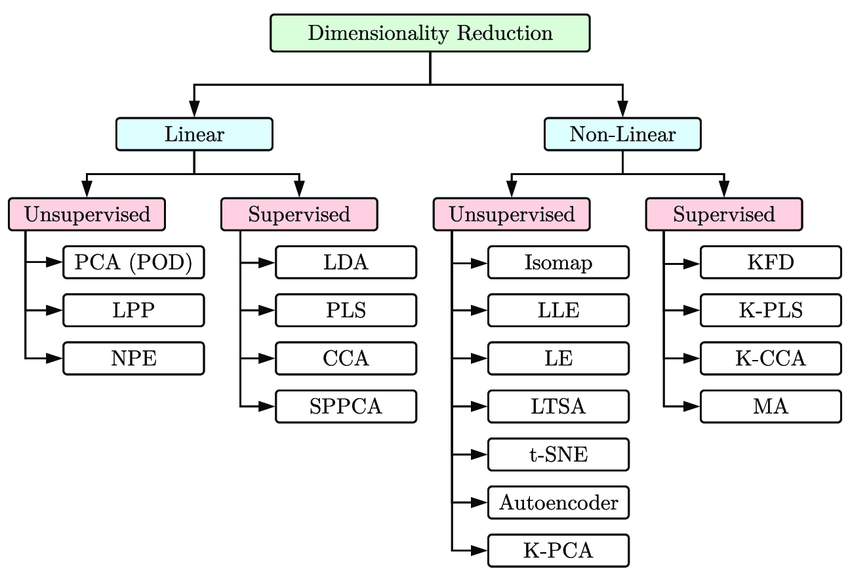
\includegraphics[width=\textwidth]{figs/dim_red_taxonomy.png}
    \caption{Таксономия методов понижения размерности}
    \label{fig:taxonomy}
\end{figure}


\section{Ответы на билеты}

\subsection{Empty space phenomenon: details and examples}

\textbf{Явление пустого пространства} -- фундаментальная проблема в геометрии высокоразмерных пространств, заключающаяся в том, что большая часть объема концентрируется вблизи границы, оставляя ``середину'' пространства практически пустой.

\subsubsection{Математическая формализация}

\paragraph{Объем гиперкуба и вписанного шара:}
   
Для $p$-мерного куба $C(R, p) = [-R, R]^p$ с объемом $V(C(R, p)) = (2R)^p$ и вписанного шара $B(R, p) = \{x \in \mathbb{R}^p: \|x\| \leq R\}$ с объемом $V(B(R, p)) = \frac{\pi^{p/2}R^p}{\Gamma(\frac{p}{2}+1)}$:
   
$$\lim_{p \to \infty} \frac{V(B(R, p))}{V(C(R, p))} = 0$$
   
Например:
\begin{itemize}
    \item При $p = 6$: отношение $\approx 0.1$ (шар занимает только 10\% объема куба)
    \item При $p = 10$: отношение $\approx 0.0025$ (0.25\%)
\end{itemize}

\paragraph{Концентрация объема на границе:}
   
Для сферической оболочки толщины $\varepsilon$ вблизи поверхности единичного шара:
   
$$\lim_{p \to \infty} \frac{V(B(1, p)) - V(B(1-\varepsilon, p))}{V(B(1, p))} = 1$$
   
Этот результат показывает, что почти весь объем шара сконцентрирован в тонком сферическом слое вблизи поверхности.

\paragraph{Диагонали гиперкуба:}
   
Для $p$-мерного куба $C(1, p) = [-1, 1]^p$, угол $\theta_p$ между любой полудиагональю $E$ (от центра до вершины) и произвольной координатной осью $E_k$:
   
$$\cos\theta_p = \frac{(E, E_k)}{\|E\| \cdot \|E_k\|} = \pm\frac{1}{\sqrt{p}}$$
   
При $p \to \infty$, $\theta_p \to \frac{\pi}{2}$, что означает: полудиагонали становятся почти ортогональными ко всем координатным осям.

\subsubsection{Последствия в анализе данных}

\begin{enumerate}
    \item \textbf{Разреженность выборки:}
    Высокоразмерное пространство $\mathbb{R}^p$ очень ``просторно'' - для покрытия значительной части объема требуется экспоненциально большое количество точек с ростом размерности $p$.

    \item \textbf{Проблемы с ближайшими соседями:}
    В высоких размерностях расстояния между точками ``выравниваются'', что усложняет различение близких и далеких соседей:
    
    $$\frac{\max_{x,y \in X} \|x-y\| - \min_{x,y \in X, x \neq y} \|x-y\|}{\min_{x,y \in X, x \neq y} \|x-y\|} \to 0 \text{ при } p \to \infty$$

    \item \textbf{Эффект проекции:}
    Проекция кластеров данных, лежащих вблизи диагоналей гиперкуба, на координатные оси приводит к их отображению вблизи начала координат, что искажает восприятие истинной структуры данных.
\end{enumerate}

\subsubsection{Примеры}

\begin{enumerate}
    \item \textbf{Равномерное распределение в гиперкубе:}
    Если $X \sim \mathcal{U}[-1,1]^p$, то вероятность, что точка находится в $\varepsilon$-окрестности центра:
    
    $$P(\|X\| \leq \varepsilon) \to 0 \text{ при } p \to \infty \text{ для любого фиксированного } \varepsilon$$

    \item \textbf{Пример с изображениями лиц:}
    Лица, описываемые векторами $10^6$ пикселей (1024×1024 изображения), занимают лишь крошечную часть всего пространства изображений, сконцентрированную вблизи некоторого многообразия низкой размерности (на практике порядка 100).

    \item \textbf{Явление в робототехнике:}
    При локализации робота по панорамному изображению (размерность 163,840), фактически изображения лежат на 3-мерном многообразии, соответствующем положению и ориентации робота.
\end{enumerate}

\subsection{Principal Component Analysis as the best linear approximation, including the solution to the Eigenvector problem}

\textbf{PCA как оптимальное линейное приближение}

Дано: высокоразмерный датасет $\{X_1, X_2, \ldots, X_n\} \subset \mathbb{R}^p$

Задача: найти линейное аффинное подпространство $L(q)$ размерности $q < p$, которое наилучшим образом аппроксимирует данные.

Формально: минимизировать функционал
$$J(L(q)) = \frac{1}{n} \sum_{i=1}^n \|X_i - \text{Pr}_{L(q)}(X_i)\|^2$$

где $\text{Pr}_{L(q)}(X_i)$ - ортогональная проекция точки $X_i$ на подпространство $L(q)$.

Решение:
\begin{enumerate}
    \item $L(q) = L(q, \bar{X}, E)$ - аффинное $q$-мерное подпространство:
    \begin{itemize}
        \item проходящее через точку $\bar{X} = \frac{1}{n}\sum_{i=1}^n X_i$ (среднее)
        \item натянутое на ортонормированные векторы $\{e_1, e_2, \ldots, e_q\}$
    \end{itemize}

    \item Ортогональная проекция: $\text{Pr}_{L(q)}(X) = \bar{X} + \sum_{k=1}^q (X-\bar{X}, e_k) \times e_k$

    \item Функционал можно переписать как:
    $$J(L(q,\bar{X}, E)) = \frac{1}{n} \sum_{i=1}^n \|X_i-\bar{X}\|^2 - \frac{1}{n} \sum_{i=1}^n \sum_{k=1}^q ((X_i-\bar{X},e_k))^2$$

    \item Минимизация $J$ эквивалентна максимизации:
    $$\Phi(E) = \frac{1}{n} \sum_{i=1}^n \sum_{k=1}^q ((X_i-\bar{X},e_k))^2 = \sum_{k=1}^q e_k^T \Sigma e_k$$
    где $\Sigma = \frac{1}{n} \sum_{i=1}^n (X_i-\bar{X})(X_i-\bar{X})^T$ - выборочная ковариационная матрица.

    \item \textbf{Решение проблемы собственных векторов}:
    \begin{itemize}
        \item Максимизация квадратичной формы $\Phi(E)$ при ограничении $E^TE = I_q$
        \item Решение: столбцы $e_1, e_2, \ldots, e_q$ матрицы $E_{PCA}$ - собственные векторы матрицы $\Sigma$, соответствующие $q$ наибольшим собственным значениям $\lambda_1 \geq \lambda_2 \geq \ldots \geq \lambda_q$
        \item $\Sigma e_k = \lambda_k e_k$, $k = 1, 2, \ldots, q$
        \item Максимальное значение функционала: $\max \Phi(E) = \sum_{k=1}^q \lambda_k$
    \end{itemize}

    \item Оптимальное подпространство: $L_{PCA}(q) = L(q, \bar{X}, E_{PCA})$
\end{enumerate}

\subsection{Principal Component Analysis from Singular Value Decomposition technique}

\textbf{PCA через сингулярное разложение (SVD)}

\begin{enumerate}
    \item Центрированная матрица данных: $\bar{\mathbf{X}} = (\bar{X}_1, \bar{X}_2, \ldots, \bar{X}_n) \in \mathbb{R}^{p \times n}$, где $\bar{X}_i = X_i - \bar{X}$

    \item Сингулярное разложение (SVD): $\bar{\mathbf{X}} = U_p \Sigma_p V_p^T$:
    \begin{itemize}
        \item $U_p$ - ортогональная $p \times p$ матрица с ортонормированными столбцами $e_1, e_2, \ldots, e_p$
        \item $\Sigma_p$ - диагональная $p \times p$ матрица с неотрицательными элементами $\sigma_1 \geq \sigma_2 \geq \ldots \geq \sigma_p$
        \item $V_p$ - ортогональная $n \times p$ матрица: $V_p^T V_p = I_p$
    \end{itemize}

    \item Связь с ковариационной матрицей:
    $$\Sigma = \frac{1}{n} \bar{\mathbf{X}} \bar{\mathbf{X}}^T = \frac{1}{n} U_p \Sigma_p^2 U_p^T$$

    \item Собственные значения и собственные векторы:
    \begin{itemize}
        \item Собственные значения ковариационной матрицы: $\lambda_k = \frac{\sigma_k^2}{n}$
        \item Собственные векторы ковариационной матрицы: столбцы $e_k$ матрицы $U_p$
    \end{itemize}

    \item PCA-представление: $Y_{PCA} = E_{PCA}^T \bar{\mathbf{X}} = \Sigma_q V_q^T$, где:
    \begin{itemize}
        \item $E_{PCA}$ - $p \times q$ матрица, составленная из первых $q$ собственных векторов $\{e_1, e_2, \ldots, e_q\}$
        \item $\Sigma_q$ - диагональная $q \times q$ матрица с первыми $q$ сингулярными числами
        \item $V_q$ - первые $q$ столбцов матрицы $V_p$
    \end{itemize}
\end{enumerate}

\subsection{Principal Component Analysis as a solution to the Dimensionality reduction problem}

\textbf{PCA как решение задачи снижения размерности}

Задача снижения размерности: найти отображения $h: \mathbb{R}^p \rightarrow \mathbb{R}^q$ и $g: \mathbb{R}^q \rightarrow \mathbb{R}^p$, минимизирующие ошибку восстановления:
$$\varepsilon(h, g) = \left(\frac{1}{n} \sum_{i=1}^n \|\hat{X}_i - X_i\|^2\right)^{1/2}$$
где $\hat{X}_i = g(h(X_i))$ - восстановленные данные.

Линейное снижение размерности:
\begin{enumerate}
    \item Линейное отображение вложения: $y_i = W(X_i - \bar{X}) \in \mathbb{R}^q$, где $W$ - ортогональная $q \times p$ матрица: $WW^T = I_q$
    
    \item Линейное отображение восстановления: $\hat{X}_i = \bar{X} + Vy_i$, где $V$ - $p \times q$ матрица

    \item Минимизация ошибки восстановления:
    \begin{itemize}
        \item Оптимальная матрица восстановления при заданной $W$: $V(W) = W^T$
        \item Восстановленное значение: $\hat{X}_i(W) = \bar{X} + W^T W (X_i - \bar{X}) = \bar{X} + P(W)(X_i - \bar{X})$
        где $P(W) = W^T W$ - ортогональная проекционная матрица: $P^T(W) = P^2(W) = P(W)$
    \end{itemize}

    \item Квадрат ошибки:
    $$\varepsilon^2(W) = \frac{1}{n}\sum_{i=1}^n \|X_i - \bar{X} - P(W)(X_i - \bar{X})\|^2 = \frac{1}{n}\sum_{i=1}^n \|X_i - \bar{X}\|^2 - \text{Tr}(W\Sigma W^T)$$

    \item Минимизация $\varepsilon^2(W)$ эквивалентна максимизации $\text{Tr}(W\Sigma W^T)$

    \item Решение: $W_{PCA} = E_{PCA}^T$, где $E_{PCA}$ - матрица собственных векторов ковариационной матрицы $\Sigma$, соответствующих $q$ наибольшим собственным значениям.
\end{enumerate}

\subsection{Principal Component Analysis as the best solution to Metric Multi Dimensionality Scaling}

\textbf{PCA как оптимальное решение метрического многомерного шкалирования (MDS)}

MDS: найти низкоразмерные представления $\{y_1, y_2, \ldots, y_n\} \subset \mathbb{R}^q$, сохраняющие попарные евклидовы расстояния:
$$\text{APD}(W) = \sum_{i,j=1}^n \left(\|X_i - X_j\|^2 - \|y_i - y_j\|^2\right)^2 \rightarrow \min$$

Учитывая, что $\|X_i - X_j\|^2 = \|X_i - \bar{X}\|^2 + \|X_j - \bar{X}\|^2 - 2(X_i - \bar{X}, X_j - \bar{X})$, задача MDS эквивалентна минимизации:
$$\text{MDS}(W) = \|\bar{\mathbf{X}}^T\bar{\mathbf{X}} - Y^TY\|_F^2$$

где $Y$ - матрица с низкоразмерными координатами: $Y = W\bar{\mathbf{X}}$

Решение SVD для матрицы $\bar{\mathbf{X}}^T\bar{\mathbf{X}}$:
$$\bar{\mathbf{X}}^T\bar{\mathbf{X}} = V_p \Sigma_p^2 V_p^T$$

Оптимальное приближение ранга $q$:
$$\bar{\mathbf{X}}^T\bar{\mathbf{X}} \approx V_q \Sigma_q^2 V_q^T = (\Sigma_q V_q^T)^T(\Sigma_q V_q^T)$$

Оптимальное решение MDS:
$$Y_{MDS} = \Sigma_q V_q^T = W_{MDS}\bar{\mathbf{X}} = W_{PCA}\bar{\mathbf{X}}$$

Таким образом, $W_{MDS} = W_{PCA}$, что показывает эквивалентность PCA и метрического MDS.

\subsection{Principal Component Analysis: as Maximum variance preserving}

\textbf{PCA как метод максимального сохранения дисперсии}

PCA можно рассматривать как поиск направлений, вдоль которых наблюдается максимальная дисперсия данных:

\begin{enumerate}
    \item Задача нахождения первой главной компоненты:
    \begin{itemize}
        \item Найти единичный вектор $e_1$, максимизирующий $\text{Var}(e_1^T X) = e_1^T \Sigma e_1$
        \item Решение: $e_1$ - собственный вектор ковариационной матрицы $\Sigma$, соответствующий наибольшему собственному значению $\lambda_1$
        \item Максимальная дисперсия: $\text{Var}(e_1^T X) = \lambda_1$
    \end{itemize}

    \item Задача нахождения $k$-ой главной компоненты $(k > 1)$:
    \begin{itemize}
        \item Найти единичный вектор $e_k$, ортогональный ко всем предыдущим $\{e_1, e_2, \ldots, e_{k-1}\}$, максимизирующий $\text{Var}(e_k^T X) = e_k^T \Sigma e_k$
        \item Решение: $e_k$ - собственный вектор матрицы $\Sigma$, соответствующий $k$-му по величине собственному значению $\lambda_k$
        \item Дисперсия $k$-ой главной компоненты: $\text{Var}(e_k^T X) = \lambda_k$
    \end{itemize}

    \item Общая дисперсия данных и доля сохраненной дисперсии:
    \begin{itemize}
        \item Полная дисперсия исходных данных: $\sum_{k=1}^p \lambda_k = \text{Tr}(\Sigma)$
        \item Дисперсия, сохраненная в первых $q$ главных компонентах: $\sum_{k=1}^q \lambda_k$
        \item Доля сохраненной дисперсии: $\frac{\sum_{k=1}^q \lambda_k}{\sum_{k=1}^p \lambda_k}$
    \end{itemize}

    \item Свойства PCA-преобразования:
    \begin{itemize}
        \item Декорреляция: $\text{Cov}(y_i, y_j) = 0$ для $i \neq j$
        \item Упорядочение по дисперсии: $\text{Var}(y_1) \geq \text{Var}(y_2) \geq \ldots \geq \text{Var}(y_q)$
        \item Оптимальность: из всех линейных преобразований, PCA обеспечивает максимальное сохранение дисперсии при заданной размерности $q$
    \end{itemize}
\end{enumerate}

\subsection{Independent component analysis: assumptions and general approach}

\textbf{Метод независимых компонент (ICA): предположения и общий подход}

ICA предполагает, что наблюдаемые данные $X \in \mathbb{R}^p$ являются линейной смесью независимых источников $S \in \mathbb{R}^q$:
$$X = AS$$

где $A$ - неизвестная $p \times q$ матрица смешивания.

\subsubsection{Основные предположения}
\begin{enumerate}
    \item Компоненты источника $s_1, s_2, \ldots, s_q$ статистически независимы: $p(s_1, s_2, \ldots, s_q) = p_1(s_1) \cdot p_2(s_2) \cdot \ldots \cdot p_q(s_q)$
    \item Не более одной компоненты может иметь гауссово распределение
    \item Число наблюдаемых сигналов не меньше числа источников: $p \geq q$
\end{enumerate}

\subsubsection{Ограничения и неоднозначности}
\begin{enumerate}
    \item Невозможно определить порядок независимых компонент
    \item Невозможно определить масштаб (дисперсию) независимых компонент
\end{enumerate}

\subsubsection{Общий подход}
\begin{enumerate}
    \item Предварительная обработка данных:
    \begin{itemize}
        \item Центрирование: $X \leftarrow X - \mathbb{E}[X]$
        \item Отбеливание: $X_V = VX$, где $V$ - матрица отбеливания: $\text{Cov}(X_V) = I$
    \end{itemize}

    \item Поиск разделяющей матрицы $W$, такой что $\hat{S} = WX$ дает оценку независимых компонент
    \begin{itemize}
        \item После отбеливания, $W$ - ортогональная матрица: $W W^T = I$
    \end{itemize}

    \item Критерии для нахождения $W$:
    \begin{itemize}
        \item Максимизация негауссовости компонент
        \item Максимизация правдоподобия
        \item Минимизация взаимной информации
    \end{itemize}

    \item Оптимизация выбранного критерия итеративными методами (градиентный спуск, FastICA)
\end{enumerate}

\subsection{Independent component analysis based on Kurtosis}

\textbf{ICA на основе куртозиса}

Куртозис как мера негауссовости случайной величины $\xi$ с $\mathbb{E}[\xi] = 0$ и $\mathbb{E}[\xi^2] = 1$:
$$\text{Kurt}(\xi) = \mathbb{E}[\xi^4] - 3(\mathbb{E}[\xi^2])^2 = \mathbb{E}[\xi^4] - 3$$

Свойства куртозиса:
\begin{itemize}
    \item Для гауссовой случайной величины: $\text{Kurt}(\text{Gauss}) = 0$
    \item Для супергауссовых распределений (с ``тяжелыми хвостами''): $\text{Kurt}(\xi) > 0$
    \item Для субгауссовых распределений: $\text{Kurt}(\xi) < 0$
\end{itemize}

Подход к ICA через максимизацию куртозиса:
\begin{enumerate}
    \item Задача: найти вектор $w$ такой, что $\hat{s} = w^T X$ имеет максимальный по модулю куртозис при $\|w\| = 1$
    \item Функционал: $F(w) = |\mathbb{E}[(w^T X)^4] - 3|$
    \item Оценка на конечной выборке: $F_n(w) = \left|\frac{1}{n}\sum_{t=1}^n (w^T X_t)^4 - 3\right|$
\end{enumerate}

Алгоритм градиентного спуска:
\begin{itemize}
    \item Если $\text{Kurt}(w^T X) > 0$: $\Delta w \propto \mathbb{E}[X (w^T X)^3]$
    \item Если $\text{Kurt}(w^T X) < 0$: $\Delta w \propto -\mathbb{E}[X (w^T X)^3]$
\end{itemize}

FastICA алгоритм (версия на основе куртозиса):
\begin{enumerate}
    \item Случайная инициализация $w$ с последующей нормализацией: $w \leftarrow w/\|w\|$
    \item Итерации:
    \begin{itemize}
        \item $w \leftarrow \mathbb{E}[X(w^T X)^3] - 3w$
        \item $w \leftarrow w/\|w\|$
    \end{itemize}
    \item Повторение итераций до сходимости
\end{enumerate}

Для нахождения нескольких независимых компонент применяется процедура декорреляции (ортогонализации Грама-Шмидта) после каждой итерации.

\subsection{Independent component analysis based on Negentropy}

\textbf{ICA на основе негэнтропии}

Негэнтропия как мера негауссовости:
$$J(\xi) = H(\xi_{\text{Gauss}}) - H(\xi)$$
где $H(\xi) = -\int p(y)\log p(y)dy$ - дифференциальная энтропия, $\xi_{\text{Gauss}}$ - гауссова случайная величина с тем же математическим ожиданием и дисперсией, что и $\xi$.

Свойства негэнтропии:
\begin{itemize}
    \item $J(\xi) \geq 0$
    \item $J(\xi) = 0$ тогда и только тогда, когда $\xi$ имеет гауссово распределение
    \item Инвариантна к линейным преобразованиям
\end{itemize}

Аппроксимации негэнтропии:
\begin{enumerate}
    \item На основе куртозиса: $J^*(\xi) = \frac{1}{12} \mathbb{E}[\xi^3]^2 + \frac{1}{48} \text{Kurt}(\xi)^2$
    \begin{itemize}
        \item Для симметричных распределений с $\mathbb{E}[\xi^3] = 0$: $J^*(\xi) = \frac{1}{48} \text{Kurt}(\xi)^2$
    \end{itemize}

    \item Аппроксимация через нелинейные функции:
    $$J^{**}(\xi) = \sum_{i=1}^m k_i[\mathbb{E}[h_i(\xi)] - \mathbb{E}[h_i(\xi_{\text{Gauss}})]^2$$
    
    Часто используемые функции:
    \begin{itemize}
        \item $h_1(y) = \frac{1}{\alpha_1} \log \cosh(\alpha_1 y)$, $1 \leq \alpha_1 \leq 2$
        \item $h_2(y) = -\exp(-y^2/2)$
    \end{itemize}
\end{enumerate}

Алгоритм FastICA на основе негэнтропии:
\begin{enumerate}
    \item Для функции $h(y) = \log \cosh(y)$ с производной $g(y) = \tanh(y)$:
    $\Delta w \propto \mathbb{E}[X g(w^T X)] - \mathbb{E}[g'(w^T X)]w$

    \item Итерации FastICA:
    \begin{itemize}
        \item $w \leftarrow \mathbb{E}[X g(w^T X)] - \mathbb{E}[g'(w^T X)]w$
        \item $w \leftarrow w/\|w\|$
    \end{itemize}

    \item Критерий сходимости: малое изменение направления $w$ между итерациями
\end{enumerate}

Сравнение с подходом на основе куртозиса:
\begin{itemize}
    \item Более устойчив к выбросам
    \item Лучше работает с распределениями разных типов
    \item Требует выбора подходящих нелинейных функций
\end{itemize}

\subsection{Independent component analysis based on Likelihood maximization and Mutual Information Minimization}

\textbf{ICA на основе максимизации правдоподобия и минимизации взаимной информации}

\subsubsection{Максимизация правдоподобия}

Плотность вероятности наблюдаемых данных при заданной разделяющей матрице $B = A^{-1}$:
$$p_X(x) = |\det(B)| \cdot \prod_{j=1}^q p_j(b_j^T x)$$
где $p_j$ - плотность вероятности $j$-й независимой компоненты.

Логарифмическая функция правдоподобия для выборки $\{X_1, X_2, \ldots, X_n\}$:
$$L(B, p_S) = \sum_{t=1}^n \sum_{i=1}^q \log p_i(b_i^T X_t) + n \log|\det(B)|$$

Максимизация $L(B, p_S)$ по $B$ (при известных или аппроксимированных $p_i$):
$$\frac{\partial L}{\partial B} = \sum_{t=1}^n g(BX_t) \cdot X_t^T + n[B^T]^{-1}$$
где $g(s) = [g_1(s_1), g_2(s_2), \ldots, g_q(s_q)]^T$, $g_i(s_i) = \frac{d}{ds_i} \log p_i(s_i)$

Итерации градиентного спуска:
$$B \leftarrow B + \eta \left(\frac{1}{n}\sum_{t=1}^n g(BX_t) \cdot X_t^T + [B^T]^{-1}\right)$$

FastICA для максимизации правдоподобия приводит к тем же обновлениям, что и в случае максимизации негэнтропии.

\subsubsection{Минимизация взаимной информации}

Взаимная информация между компонентами $s_1, s_2, \ldots, s_q$:
$$I(s_1, s_2, \ldots, s_q) = \sum_{i=1}^q H(s_i) - H(s_1, s_2, \ldots, s_q)$$

Свойства:
\begin{itemize}
    \item $I(s_1, s_2, \ldots, s_q) \geq 0$ 
    \item $I(s_1, s_2, \ldots, s_q) = 0$ тогда и только тогда, когда $s_1, s_2, \ldots, s_q$ статистически независимы
\end{itemize}

Для преобразования $S = BX$:
$$I(s_1, s_2, \ldots, s_q) = \sum_{i=1}^q H(s_i) - H(X) - \log|\det(B)|$$

Для ортогональной матрицы $B$ после отбеливания:
$$I(s_1, s_2, \ldots, s_q) = \sum_{i=1}^q H(s_i) - H(X)$$

Минимизация взаимной информации эквивалентна минимизации суммы энтропий отдельных компонент, что в свою очередь эквивалентно максимизации суммы негэнтропий компонент.

Эквивалентность подходов:
\begin{itemize}
    \item Максимизация правдоподобия
    \item Минимизация взаимной информации (при правильном выборе функций)
    \item Максимизация негауссовости через негэнтропию
\end{itemize}

Это показывает, что различные формулировки ICA приводят к одним и тем же алгоритмам, хотя и с разных теоретических позиций.

\subsection{Projection pursuit: an approach and examples}

\textbf{Projection Pursuit: подход и примеры}

Projection Pursuit (преследование проекций) - методы, которые ищут интересные низкоразмерные линейные проекции многомерных данных путем оптимизации определенной целевой функции, называемой индексом проекции.

\subsubsection{Общий подход}
\begin{enumerate}
    \item Выбор индекса проекции $I(b)$, который измеряет ``интересность'' проекции данных на направление $b$, $\|b\| = 1$
    \item Поиск направления $b^*$, максимизирующего выбранный индекс: $b^* = \arg\max_b I(b)$
    \item Для многомерных проекций: последовательный или одновременный поиск нескольких направлений
\end{enumerate}

\subsubsection{Примеры индексов проекции}

\begin{enumerate}
    \item \textbf{Дисперсия} (приводит к PCA):
   $$I_{PCA}(b) = \text{Var}(b^T X) = b^T \Sigma b$$

    \item \textbf{Куртозис} (приводит к одному из вариантов ICA):
   $$I_{ICA-1}(b) = |\text{Kurt}(b^T X)| = |E[(b^T X)^4] - 3(E[(b^T X)^2])^2|$$

    \item \textbf{Негэнтропия} (другой вариант ICA):
   $$I_{ICA-2}(b) = J(b^T X) \approx [E[G(b^T X)] - E[G(\xi_{Gauss})]]^2$$
   где $G$ - некоторая нелинейная функция, $\xi_{Gauss}$ - стандартная гауссова случайная величина.

    \item \textbf{Энтропия} (минимизация вместо максимизации):
   $$I_H(b) = -H(b^T X)$$

    \item \textbf{Индекс Фридмана-Таки} (оригинальная мера ``дырчатости''):
   $$I_{FT}(b) = \sum_{i=1}^n\sum_{j=1}^n [f(b^T (X_i - X_j)) - f_0]^2$$
   где $f$ - гауссово ядро, $f_0$ - константа нормализации.

    \item \textbf{Индекс для дискриминантного анализа:}
   $$I_{LDA}(b) = \frac{b^T \Sigma_{between} b}{b^T \Sigma_{within} b}$$
\end{enumerate}

\subsubsection{Примеры применения}

\begin{enumerate}
    \item \textbf{Кластерный анализ}: поиск проекций, выявляющих кластерную структуру данных
    \begin{itemize}
        \item Проекции, максимизирующие индексы на основе смеси распределений
        \item Визуализация мультимодальных данных
    \end{itemize}

    \item \textbf{Выявление выбросов}: направления, максимизирующие асимметрию или куртозис

    \item \textbf{Исследование нелинейных структур}: направления, максимизирующие любые отклонения от нормальности

    \item \textbf{Дискриминантный анализ}: направления, максимизирующие разделение классов
    \begin{itemize}
        \item LDA как частный случай Projection Pursuit
    \end{itemize}

    \item \textbf{Классификация банкнот (швейцарский пример)}: обнаружение подделок через проекции, максимизирующие индекс ``Hermit''

    \item \textbf{Анализ многомерных данных}: поиск интересных зависимостей в сложных наборах данных
    \begin{itemize}
        \item Например, выявление бивариантной смеси двух гауссианов в 10-мерном зашумленном пространстве
    \end{itemize}
\end{enumerate}

\subsubsection{Оптимизация индексов проекции}
\begin{enumerate}
    \item Для некоторых индексов (PCA, LDA) - аналитическое решение через собственные значения
    \item Для других индексов - численные методы оптимизации:
    \begin{itemize}
        \item Градиентный спуск
        \item Методы Ньютона
        \item Методы поиска без производных
    \end{itemize}
\end{enumerate}

PCA и ICA можно рассматривать как частные случаи Projection Pursuit с конкретными индексами проекции.

\section{Внутренняя размерность (Intrinsic Dimension)}

\subsection{Математические определения внутренней размерности}

\textbf{Внутренняя размерность} характеризует минимальное число параметров, необходимых для описания данных без потери информации. Существует несколько формальных математических определений:

\subsubsection{Размерность Хаусдорфа}

Для ограниченного множества $C \subset \mathbb{R}^p$ и $S(X, r)$ - $r$-шара с центром в $X$:

Пусть $S(r) = \{S(X_i, r_i)\}$ - набор шаров такой, что:
\begin{itemize}
    \item $r_i \leq r$
    \item $\cup_i S(X_i, r_i) \supset C$
\end{itemize}

Определяем величину:
\begin{equation}
    H_r^d = \inf_S \sum_i r_i^d
\end{equation}

где инфимум берется по всем возможным покрытиям $S$.

\textbf{Размерность Хаусдорфа $D_H$} определяется как критическое значение:
\begin{equation}
    H^d = \lim_{r \to 0} H_r^d = \begin{cases}
    \infty, & \text{если } d < D_H \\
    0, & \text{если } d > D_H \\
    \text{константа} \neq 0, & \text{если } d = D_H
    \end{cases}
\end{equation}

\paragraph{Пример:}
Для отрезка $C = [0, 1]$ при $r = 1/(2n)$:
\begin{equation}
    H_r^d = \sum_{i=1}^n \left(\frac{1}{2n}\right)^d = \frac{1}{2^d} \cdot n^{1-d}
\end{equation}

Откуда следует $D_H = 1$.

\subsubsection{Колмогоровская ёмкость (Box-counting dimension)}

Для множества $C \subset \mathbb{R}^p$ обозначим $N(C, r)$ - минимальное число шаров радиуса $r$, необходимых для покрытия $C$.

\textbf{Ёмкостная размерность} определяется как:
\begin{equation}
    D_{Cap} = \lim_{r \to 0} \frac{\ln N(C, r)}{\ln \frac{1}{r}}
\end{equation}

Для отрезка $C = [0, 1]$ при $r = 1/(2n)$: $N(C, r) = n$, откуда $D_{Cap} = 1$.

\subsubsection{Размерность Хаусдорфа-Безиковича}

Пусть $E_r = \{[kr, kr + r)^p, k = 0, \pm 1, \pm 2, \ldots\}$ - множество кубов в $\mathbb{R}^p$ с ребром $r$.

Обозначим $N(C, r) = \#\{Q \in E_r: C \cap Q \neq \emptyset\}$ - число кубов, пересекающихся с $C$.

Если существуют числа $V$ и $D$ такие, что:
\begin{equation}
    \lim_{r \to 0} \frac{N(C, r)}{V \cdot r^{-D}} = 1
\end{equation}

то $D_{HB}(C) = D$ называется \textbf{размерностью Хаусдорфа-Безиковича}, а $V_{HB}(C) = V$ - соответствующим объемом.

Если $C$ измеримо по Жордану, то $D_{HB}(C)$ и $V_{HB}(C)$ равны топологической размерности и объему соответственно.

\subsubsection{Корреляционная размерность}

Пусть $\{X_1, X_2, \ldots, X_n\}$ - выборка из $C$, а $m(n) = n(n-1)/2$ - число пар.

\textbf{Корреляционный интеграл}:
\begin{equation}
    C_n(r) = \frac{1}{m(n)} \sum_{1 \leq i < j \leq n} I(||X_i - X_j|| \leq r)
\end{equation}

где $I(A)$ - индикатор события $A$.

\textbf{Корреляционная размерность} определяется как:
\begin{equation}
    D_{corr} = \lim_{r \to 0} \frac{\ln C_n(r)}{\ln r}
\end{equation}

при $n \to \infty$.

\subsubsection{Взаимосвязь размерностей}

Для "хороших" множеств эти размерности совпадают, но в общем случае:
\begin{equation}
    D_{corr} \leq D_{HB} \leq D_{Cap} \leq D_H
\end{equation}

Эти определения имеют теоретическое значение, но напрямую их сложно использовать для оценки размерности по конечной выборке данных.

\subsection{Оценка внутренней размерности: геометрические методы}

Геометрические методы оценки внутренней размерности основаны на анализе пространственных отношений между точками выборки.

\subsubsection{Методы на основе адаптации математических определений}

\paragraph{Метод оценки корреляционной размерности}

Для конечной выборки {$X_1, X_2, \ldots, X_n$} вычисляется корреляционный интеграл для различных значений $r$:
\begin{equation}
    C_n(r) = \frac{1}{m(n)} \sum_{1 \leq i < j \leq n} I(||X_i - X_j|| \leq r)
\end{equation}

График зависимости $\ln C_n(r)$ от $\ln r$ аппроксимируется прямой линией, наклон которой дает оценку размерности:
\begin{equation}
    D_{corr} \approx \frac{\ln C_n(r_2) - \ln C_n(r_1)}{\ln r_2 - \ln r_1}
\end{equation}

\textbf{Практическая реализация:}
\begin{enumerate}
    \item Вычислить $C_n(r)$ для нескольких значений $r$
    \item Построить график $\ln C_n(r)$ от $\ln r$
    \item Найти линейный участок и определить его наклон
\end{enumerate}

\paragraph{Box-counting метод}

\begin{enumerate}
    \item Разбить пространство сеткой с размером ячейки $r$
    \item Подсчитать число ячеек $N(r)$, содержащих хотя бы одну точку выборки
    \item Построить график зависимости $\ln N(r)$ от $\ln (1/r)$
    \item Определить наклон линейного участка как оценку размерности:
    \begin{equation}
        D_{Cap} \approx \frac{\ln N(r_2) - \ln N(r_1)}{\ln (1/r_2) - \ln (1/r_1)}
    \end{equation}
\end{enumerate}

\subsubsection{Метод PCA и его локальные вариации}

\paragraph{Глобальный PCA}

\begin{enumerate}
    \item Вычислить ковариационную матрицу $\Sigma = \frac{1}{n} \sum_{i=1}^n (X_i - \bar{X})(X_i - \bar{X})^T$
    \item Найти собственные значения $\lambda_1 \geq \lambda_2 \geq \ldots \geq \lambda_p$
    \item Оценить размерность как число значимых собственных значений:
    \begin{equation}
        D_{PCA} = \min\left\{q: \frac{\sum_{k=1}^q \lambda_k}{\sum_{k=1}^p \lambda_k} > \text{threshold}\right\}
    \end{equation}
\end{enumerate}

где threshold обычно выбирается как 0.9 или 0.95.

\paragraph{Локальный PCA}

\begin{enumerate}
    \item Для каждой точки $X_i$ найти ее окрестность $U(X_i)$ (k ближайших соседей или $\epsilon$-окрестность)
    \item Применить PCA к каждой окрестности $U(X_i)$, получив локальные собственные значения $\{\lambda_{i1}, \lambda_{i2}, \ldots, \lambda_{ip}\}$
    \item Усреднить собственные значения по всем точкам: $\lambda_t = \frac{1}{n} \sum_{i=1}^n \lambda_{it}$
    \item Оценить размерность аналогично глобальному PCA:
    \begin{equation}
        D_{LPCA} = \min\left\{q: \frac{\sum_{k=1}^q \lambda_k}{\sum_{k=1}^p \lambda_k} > \text{threshold}\right\}
    \end{equation}
\end{enumerate}

\subsubsection{Метод на основе углов между векторами}

\begin{enumerate}
    \item Для каждой точки $X_i$ найти ее k ближайших соседей $X_{(1)}, X_{(2)}, \ldots, X_{(k)}$
    \item Построить подпространство $L(X_i, k) = \text{Span}(X_{(1)}-X_i, X_{(2)}-X_i, \ldots, X_{(k)}-X_i)$
    \item Измерить угол $\alpha_i^{(k)}$ между вектором $X_{(k+1)}-X_i$ к $(k+1)$-му соседу и его проекцией на $L(X_i, k)$
    \item Увеличивать $k$ пока средний угол $\bar{\alpha}^{(k)} = \frac{1}{n} \sum_{i=1}^n \alpha_i^{(k)}$ не превысит выбранный порог
    \item Оценка размерности: $D = \min\{k: \bar{\alpha}^{(k)} < \text{threshold}\}$
\end{enumerate}

\subsubsection{Метод на основе собственных значений оператора Лапласа}

Для графа соседства с весами $W_{ij}$:
\begin{enumerate}
    \item Построить матрицу Лапласа $L = D - W$, где $D$ - диагональная матрица степеней
    \item Найти собственные значения $0 = \mu_1 \leq \mu_2 \leq \ldots \leq \mu_n$
    \item Применить асимптотическую формулу: $\log(\mu_j) \approx A + \frac{2}{q}\log(j)$, где $q$ - внутренняя размерность
    \item Оценить размерность методом регрессии из соотношения:
    \begin{equation}
        D_{Lap} \approx \frac{2}{\text{наклон графика } \log(\mu_j) \text{ от } \log(j)}
    \end{equation}
\end{enumerate}

\subsubsection{Преимущества и недостатки геометрических методов}

\paragraph{Преимущества:}
\begin{itemize}
    \item Интуитивная геометрическая интерпретация
    \item Некоторые методы не требуют явных предположений о распределении данных
    \item Возможность анализировать локальную размерность в разных частях данных
\end{itemize}

\paragraph{Недостатки:}
\begin{itemize}
    \item Чувствительность к выбору параметров (размеру окрестности, порогу)
    \item Проблемы с масштабируемостью на больших наборах данных
    \item Некоторые методы чувствительны к шуму и выбросам
\end{itemize}

\subsection{Оценка внутренней размерности: регрессионный подход}

Регрессионные методы оценки внутренней размерности основаны на моделировании отношений между расстояниями до ближайших соседей и их количеством или рангом.

\subsubsection{Теоретическое обоснование}

Пусть $X$ - многообразие с внутренней размерностью $d$, вложенное в $\mathbb{R}^p$, с плотностью вероятности $f(X)$.

Для малого шара $B(X, \varepsilon)$ с центром в точке $X \in X$ и радиусом $\varepsilon$:

Вероятность, что случайная точка $X'$ попадет в этот шар:
\begin{equation}
    P(X, \varepsilon) = P(X' \in B(X, \varepsilon) \cap X) \approx f(X) \cdot \varepsilon^d \cdot V(d)
\end{equation}

где $V(d) = \frac{\pi^{d/2}}{\Gamma(\frac{d}{2}+1)}$ - объем $d$-мерного единичного шара.

\subsubsection{Метод регрессии на k ближайших соседях}

\begin{enumerate}
    \item Для каждой точки $X_i$ из выборки $\{X_1, X_2, \ldots, X_n\}$:
    \begin{itemize}
        \item Найти $k$ ближайших соседей $X_{(1)}, X_{(2)}, \ldots, X_{(k)}$
        \item Вычислить расстояния $r_j(X_i) = \|X_{(j)} - X_i\|$ для $j = 1, 2, \ldots, k$
    \end{itemize}

    \item Для шара $B(X_i, r_k(X_i))$ точно $k$ точек из $n$ попадает внутрь, следовательно:
    \begin{equation}
        \frac{k}{n} \approx P(X_i, r_k(X_i)) \approx f(X_i) \cdot (r_k(X_i))^d \cdot V(d)
    \end{equation}

    \item Логарифмируя обе части:
    \begin{equation}
        \ln k - \ln n \approx \ln f(X_i) + d \cdot \ln r_k(X_i) + \ln V(d)
    \end{equation}

    \item Перегруппировав:
    \begin{equation}
        \ln k \approx A_i + d \cdot T_k(i)
    \end{equation}
    
    где $A_i = A_i(d) = \ln n - \ln V(d) - \ln f(X_i)$ и $T_k(i) = -\ln r_k(X_i)$

    \item Для каждой точки $X_i$ и различных значений $k$ получается система регрессионных уравнений:
    \begin{equation}
        \ln k \approx A_i + d \cdot T_k(i), \quad k = 1, 2, \ldots, k_{max}
    \end{equation}

    \item Оценка размерности получается методом наименьших квадратов:
    \begin{equation}
        d = \frac{\sum_{i=1}^n \sum_{k=1}^{k_{max}} (T_k(i) - \bar{T}_i)(\ln k - \overline{\ln k})}{\sum_{i=1}^n \sum_{k=1}^{k_{max}} (T_k(i) - \bar{T}_i)^2}
    \end{equation}

    где $\bar{T}_i = \frac{1}{k_{max}} \sum_{k=1}^{k_{max}} T_k(i)$ и $\overline{\ln k} = \frac{1}{k_{max}} \sum_{k=1}^{k_{max}} \ln k$.
\end{enumerate}

\subsubsection{Вариации регрессионного подхода}

\paragraph{Метод Levina-Bickel (2005)}

Для каждой точки $X_i$ строится локальная оценка:
\begin{equation}
    \hat{d}_i = \left( \frac{1}{k} \sum_{j=1}^k \ln \frac{r_k(X_i)}{r_j(X_i)} \right)^{-1}
\end{equation}

Глобальная оценка получается усреднением:
\begin{equation}
    \hat{d} = \frac{1}{n} \sum_{i=1}^n \hat{d}_i
\end{equation}

\paragraph{Метод построения кривой масштабирования}

\begin{enumerate}
    \item Вычислить среднее расстояние до $k$-ого соседа:
    \begin{equation}
        \bar{r}_k = \frac{1}{n} \sum_{i=1}^n r_k(X_i)
    \end{equation}

    \item Построить зависимость $\ln \bar{r}_k$ от $\ln k$
    \item Наклон этой зависимости равен $1/d$:
    \begin{equation}
        \hat{d} = \frac{\ln k_2 - \ln k_1}{\ln \bar{r}_{k_2} - \ln \bar{r}_{k_1}}
    \end{equation}
\end{enumerate}

\subsubsection{Практические соображения}

\begin{enumerate}
    \item \textbf{Выбор значения $k$}:
    \begin{itemize}
        \item При малых $k$ оценки нестабильны из-за локальных флуктуаций
        \item При больших $k$ могут нарушаться предположения о локальной линейности многообразия
        \item Рекомендуется анализировать устойчивость оценки при различных $k$
    \end{itemize}

    \item \textbf{Робастность}:
    \begin{itemize}
        \item Для повышения устойчивости к выбросам можно использовать медианное усреднение вместо среднего
        \item Возможно применение робастных методов регрессии
    \end{itemize}

    \item \textbf{Коррекция смещения}:
    \begin{itemize}
        \item При малом размере выборки методы могут давать смещенные оценки
        \item Предложены различные методы коррекции смещения, например, путем введения поправочных коэффициентов
    \end{itemize}
\end{enumerate}

\subsubsection{Преимущества и недостатки регрессионного подхода}

\paragraph{Преимущества:}
\begin{itemize}
    \item Статистически обоснованные оценки
    \item Возможность получения локальных оценок размерности
    \item Относительная простота реализации
\end{itemize}

\paragraph{Недостатки:}
\begin{itemize}
    \item Чувствительность к выбору параметров (особенно $k$)
    \item Предположение о равномерном распределении точек в локальных окрестностях
    \item Проблемы со сходимостью при наличии шума или неравномерной выборки
\end{itemize}

\subsection{Оценка внутренней размерности: подход максимального правдоподобия}

Метод максимального правдоподобия (MLE) для оценки внутренней размерности основан на моделировании локального распределения расстояний между точками данных.

\subsubsection{Теоретическое обоснование}

Предположения:
\begin{enumerate}
    \item Данные лежат на или вблизи многообразия размерности $d$ в $\mathbb{R}^p$
    \item Локально многообразие можно аппроксимировать евклидовым пространством $\mathbb{R}^d$
    \item Точки выборки распределены локально равномерно с плотностью $f(X)$
\end{enumerate}

\subsubsection{Метод Levina-Bickel (2005)}

\paragraph{Вероятностная модель}

В окрестности точки $X$ вероятность обнаружить точку на расстоянии от $t$ до $t + dt$ моделируется пуассоновским процессом с интенсивностью:
\begin{equation}
    \lambda(t) = f(X) \cdot V(d) \cdot d \cdot t^{d-1}
\end{equation}

где:
\begin{itemize}
    \item $f(X)$ - плотность в точке $X$
    \item $V(d) = \frac{\pi^{d/2}}{\Gamma(\frac{d}{2}+1)}$ - объем $d$-мерного единичного шара
    \item $d \cdot t^{d-1}$ - производная от $t^d$
\end{itemize}

\paragraph{Функция правдоподобия}

Для точки $X$ и ее соседей на расстояниях $r_1 < r_2 < \ldots < r_k$ функция правдоподобия:
\begin{equation}
    F(f(X), d) = \exp\left(\int_0^{r_k} \ln \lambda(t) dN(X, t) - \int_0^{r_k} \lambda(t) dt\right)
\end{equation}

где $N(X, t)$ - число точек в шаре радиуса $t$ с центром в $X$.

При дифференцировании по $t$, интеграл преобразуется в сумму:
\begin{equation}
    \ln F(f(X), d) = \sum_{j=1}^{k-1} \ln\lambda(r_j) - \int_0^{r_k} \lambda(t) dt
\end{equation}

\paragraph{Максимизация правдоподобия}

Оценка максимального правдоподобия для размерности $d$ в точке $X$ при $R = r_k$:
\begin{equation}
    D_R(X) = \left(\frac{1}{k-1} \sum_{j=1}^{k-1} \ln\frac{R}{r_j} \right)^{-1}
\end{equation}

Используя $k$ ближайших соседей и обозначая $R = r_k(X)$:
\begin{equation}
    D_k(X) = \left(\frac{1}{k-1} \sum_{j=1}^{k-1} \ln\frac{r_k(X)}{r_j(X)} \right)^{-1}
\end{equation}

Глобальная оценка получается усреднением по всем точкам:
\begin{equation}
    D_k = \frac{1}{n} \sum_{i=1}^n D_k(X_i)
\end{equation}

\subsubsection{Расширения метода MLE}

\paragraph{MLE с переменным $k$ (Levina-Bickel, 2005)}

Для улучшения устойчивости оценки:
\begin{equation}
    D_{k_1, k_2} = \frac{1}{n} \sum_{i=1}^n \frac{1}{k_2 - k_1 + 1} \sum_{k=k_1}^{k_2} D_k(X_i)
\end{equation}

\paragraph{MLE с коррекцией смещения (Mackay-Ghahramani, 2005)}

Учитывает систематическое смещение при малых $k$:
\begin{equation}
    D_k^{corrected} = \frac{k-2}{k-1} \cdot D_k
\end{equation}

\paragraph{Геодезический MLE (Chen et al., 2013)}

Заменяет евклидовы расстояния на геодезические для улучшения оценки на искривленных многообразиях:
\begin{equation}
    D_k^{geo}(X) = \left(\frac{1}{k-1} \sum_{j=1}^{k-1} \ln\frac{d_{geo}(X, X_{(k)})}{d_{geo}(X, X_{(j)})} \right)^{-1}
\end{equation}

где $d_{geo}(X, Y)$ - аппроксимация геодезического расстояния (например, через графовые расстояния).

\subsubsection{Оценка плотности}

MLE также позволяет оценить локальную плотность $f(X)$:
\begin{equation}
    \hat{f}_R(X) = \frac{k-1}{V(D_R(X)) \cdot R^{D_R(X)}}
\end{equation}

или при использовании $k$ ближайших соседей:
\begin{equation}
    \hat{f}_k(X) = \frac{k-1}{V(D_k(X)) \cdot (r_k(X))^{D_k(X)}}
\end{equation}

Это позволяет оценить энтропию распределения:
\begin{equation}
    \hat{J}(f) = \frac{1}{n} \sum_{i=1}^n \ln(\hat{f}_k(X_i))
\end{equation}

\subsubsection{Выбор оптимального $k$}

Ключевой вопрос - как выбрать оптимальное значение $k$. Предложены различные подходы:

\begin{enumerate}
    \item \textbf{Метод стабилизации}: выбрать $k$, при котором оценка $D_k$ стабилизируется

    \item \textbf{Метод минимальной вариации}: минимизировать дисперсию локальных оценок $D_k(X_i)$

    \item \textbf{Кросс-валидация}: оптимизировать прогностическую способность модели

    \item \textbf{Байесовский подход}: усреднить оценки с различными $k$ с соответствующими весами
\end{enumerate}

\subsubsection{Преимущества и недостатки подхода MLE}

\paragraph{Преимущества:}
\begin{itemize}
    \item Статистически обоснованный метод с теоретическими гарантиями
    \item Возможность получения как локальных, так и глобальных оценок
    \item Одновременная оценка размерности и плотности
    \item Высокая эффективность на данных, близких к предположениям модели
\end{itemize}

\paragraph{Недостатки:}
\begin{itemize}
    \item Предположение о локально равномерном распределении данных
    \item Чувствительность к выбору числа соседей $k$
    \item Вычислительные затраты на поиск $k$ ближайших соседей
    \item Потенциальные проблемы на границах многообразия
\end{itemize}

\subsubsection{Практические рекомендации:}

\begin{enumerate}
    \item Использовать несколько значений $k$ и анализировать стабильность оценки
    \item Сравнивать результаты с другими методами оценки размерности
    \item Визуализировать локальные оценки для выявления областей с различной локальной размерностью
    \item При наличии шума, предварительно применять методы его подавления
\end{enumerate}

MLE подход к оценке внутренней размерности является одним из наиболее теоретически обоснованных и широко используемых на практике.


\section{Методы обучения многообразий (Manifold Learning)}

\subsection{Locally Linear Embedding (LLE)}

\textbf{Локально-линейное вложение (LLE)} -- метод нелинейного снижения размерности, сохраняющий локальную геометрию данных путем представления точек как линейных комбинаций их соседей.

\subsubsection{Теоретическое обоснование}

LLE основан на предположении, что локально (в малой окрестности) многообразие можно аппроксимировать линейным подпространством. Следовательно, каждая точка может быть представлена как линейная комбинация своих ближайших соседей.

\subsubsection{Алгоритм LLE}

\begin{enumerate}
    \item \textbf{Определение соседства}:
    \begin{itemize}
        \item Для каждой точки $X_i \in \mathbb{R}^p$ найти $k$ ближайших соседей $\{X_1(i), X_2(i), \ldots, X_k(i)\}$
    \end{itemize}
    
    \item \textbf{Вычисление весовых коэффициентов}:
    \begin{itemize}
        \item Для каждой точки $X_i$ найти веса $\{w_1(i), w_2(i), \ldots, w_k(i)\}$, которые минимизируют:
        \begin{equation}
            E_i = \left\|X_i - \sum_{j=1}^k w_j(i) \times X_j(i)\right\|^2
        \end{equation}
        \item При условии: $\sum_{j=1}^k w_j(i) = 1$ (для инвариантности к сдвигам)
        \item Решение находится аналитически через систему линейных уравнений:
        \begin{align}
            G_{ts}(i) &= (X_t(i) - X_i) \cdot (X_s(i) - X_i) \\
            w_t(i) &= \frac{\sum_{s=1}^k G_{ts}^{-1}(i)}{\sum_{t,s=1}^k G_{ts}^{-1}(i)}
        \end{align}
    \end{itemize}
    
    \item \textbf{Построение низкоразмерного вложения}:
    \begin{itemize}
        \item Найти $q$-мерные координаты $\{y_1, y_2, \ldots, y_n\} \subset \mathbb{R}^q$, минимизирующие:
        \begin{equation}
            \Phi(Y) = \sum_{i=1}^n \left\|y_i - \sum_{j=1}^k w_j(i) \times y_j(i)\right\|^2
        \end{equation}
        \item С ограничениями: $\frac{1}{n}\sum_{i=1}^n y_i = 0$ и $\frac{1}{n}\sum_{i=1}^n y_i y_i^T = I_q$
        \item В матричной форме: $L(Y) = \text{Tr}(Y(I_n-W)^T(I_n-W)Y^T)$
    \end{itemize}
    
    \item \textbf{Решение задачи собственных значений}:
    \begin{itemize}
        \item Минимизация $L(Y)$ эквивалентна нахождению $q$ собственных векторов матрицы:
        \begin{equation}
            M_{LLE} = (I_n-W)^T(I_n-W)
        \end{equation}
        \item соответствующих $q$ наименьшим ненулевым собственным значениям
        \item Собственный вектор с нулевым собственным значением (константный) отбрасывается
    \end{itemize}
\end{enumerate}

\subsubsection{Преимущества и недостатки LLE}

\paragraph{Преимущества:}
\begin{itemize}
    \item Сохраняет локальную структуру данных
    \item Требует настройки всего одного параметра (числа соседей $k$)
    \item Имеет аналитическое решение (задача собственных значений)
    \item Эффективно работает для данных, лежащих на гладком многообразии
\end{itemize}

\paragraph{Недостатки:}
\begin{itemize}
    \item Чувствителен к выбору числа соседей $k$
    \item Может давать топологические "сшивания" и "складки" при сложной геометрии данных
    \item Плохо работает с негладкими многообразиями или при наличии "дыр"
    \item Не всегда хорошо сохраняет глобальную структуру данных
    \item Проблемы с масштабируемостью для очень больших наборов данных
\end{itemize}

\subsection{ISOmetric MAPping (ISOMAP)}

\textbf{ISOmetric MAPping (ISOMAP)} -- метод нелинейного снижения размерности, который сохраняет геодезические расстояния между точками многообразия.

\subsubsection{Теоретическое обоснование}

ISOMAP основан на предположении, что евклидовы расстояния в исходном пространстве не отражают истинную структуру нелинейного многообразия. Вместо них используются геодезические расстояния -- длины кратчайших путей по многообразию.

\subsubsection{Алгоритм ISOMAP}

\begin{enumerate}
    \item \textbf{Построение графа соседства}:
    \begin{itemize}
        \item Для каждой точки $X_i$ определить соседей (через $k$ ближайших соседей или $\epsilon$-окрестность)
        \item Построить взвешенный неориентированный граф $\Gamma(X_n)$, где веса рёбер равны евклидовым расстояниям между соседними точками
    \end{itemize}
    
    \item \textbf{Вычисление геодезических расстояний}:
    \begin{itemize}
        \item Используя алгоритм Дейкстры (или Флойда-Уоршалла), найти длины кратчайших путей $D(X_i, X_j)$ между всеми парами точек в графе
        \item Эти расстояния аппроксимируют геодезические расстояния на многообразии
    \end{itemize}
    
    \item \textbf{Применение многомерного шкалирования (MDS)}:
    \begin{itemize}
        \item Построить матрицу квадратов расстояний $\mathbf{D}_X$ с элементами $[D(X_i, X_j)]^2$
        \item Выполнить операцию двойного центрирования: $\mathbf{S}_X = -\frac{1}{2}H\mathbf{D}_XH$, где $H = I_n - \frac{1}{n}\mathbf{1}\mathbf{1}^T$ -- центрирующая матрица
        \item Найти $q$ собственных векторов $v_1, v_2, \ldots, v_q$ матрицы $\mathbf{S}_X$, соответствующих $q$ наибольшим собственным значениям $\lambda_1 \geq \lambda_2 \geq \ldots \geq \lambda_q$
        \item $q$-мерные координаты: $Y = \Lambda^{1/2}V^T$, где $\Lambda = \text{diag}(\lambda_1, \lambda_2, \ldots, \lambda_q)$ и $V = [v_1, v_2, \ldots, v_q]$
    \end{itemize}
\end{enumerate}

\subsubsection{Теоретические гарантии}

Если многообразие изометрично евклидову пространству, то при достаточно плотной выборке и правильном выборе параметров ISOMAP гарантированно восстанавливает истинную геометрию многообразия с точностью до изометрии.

\subsubsection{Преимущества и недостатки ISOMAP}

\paragraph{Преимущества:}
\begin{itemize}
    \item Сохраняет глобальную геометрическую структуру данных
    \item Теоретически обоснован для изометрично вложенных многообразий
    \item Интуитивно понятный подход через геодезические расстояния
    \item Хорошо работает для данных, лежащих на "развертываемых" многообразиях
\end{itemize}

\paragraph{Недостатки:}
\begin{itemize}
    \item Чувствителен к шуму и выбросам
    \item Требует точной аппроксимации геодезических расстояний
    \item Проблемы с "дырами" в данных и негладкими многообразиями
    \item Вычислительно затратен для больших наборов данных (O(n³) для MDS)
    \item Ограничен многообразиями, которые можно изометрически отобразить в евклидово пространство
\end{itemize}

\subsection{Laplacian Eigenmaps}

\textbf{Laplacian Eigenmaps (собственные карты Лапласа)} -- метод нелинейного снижения размерности, основанный на теории спектральных графов и дифференциальной геометрии.

\subsubsection{Теоретическое обоснование}

Метод основан на связи между лапласианом графа и оператором Лапласа-Бельтрами на многообразии. Основная идея заключается в том, что собственные функции оператора Лапласа-Бельтрами образуют оптимальное вложение многообразия, сохраняющее его локальную структуру.

\subsubsection{Алгоритм Laplacian Eigenmaps}

\begin{enumerate}
    \item \textbf{Построение графа соседства}:
    \begin{itemize}
        \item Для каждой точки $X_i$ определить соседей (через $k$ ближайших соседей или $\epsilon$-окрестность)
        \item Построить неориентированный граф $\Gamma(X_n)$, где рёбра соединяют соседние точки
    \end{itemize}
    
    \item \textbf{Взвешивание рёбер} (опционально):
    \begin{itemize}
        \item Определить веса рёбер, например, используя тепловое ядро:
        \begin{equation}
            W_{ij} = \begin{cases}
            \exp\left(-\frac{\|X_i - X_j\|^2}{t}\right), & \text{если } X_i \text{ и } X_j \text{ соседи} \\
            0, & \text{иначе}
            \end{cases}
        \end{equation}
        \item Где $t > 0$ -- параметр ширины ядра
    \end{itemize}
    
    \item \textbf{Построение лапласиана графа}:
    \begin{itemize}
        \item Вычислить матрицу степеней $D$ -- диагональную матрицу с элементами $D_{ii} = \sum_j W_{ij}$
        \item Построить лапласиан $L = D - W$
    \end{itemize}
    
    \item \textbf{Спектральное разложение}:
    \begin{itemize}
        \item Решить обобщённую задачу собственных значений:
        \begin{equation}
            L v = \lambda D v
        \end{equation}
        \item Отбросить собственный вектор $v_0$, соответствующий нулевому собственному значению $\lambda_0 = 0$
        \item Использовать $q$ собственных векторов $v_1, v_2, \ldots, v_q$, соответствующих $q$ наименьшим ненулевым собственным значениям $\lambda_1 \leq \lambda_2 \leq \ldots \leq \lambda_q$, для формирования $q$-мерного вложения:
        \begin{equation}
            y_i = (v_{1i}, v_{2i}, \ldots, v_{qi})^T, \quad i = 1, 2, \ldots, n
        \end{equation}
    \end{itemize}
\end{enumerate}

\subsubsection{Связь с оператором Лапласа-Бельтрами}

Дискретный лапласиан $L$ аппроксимирует оператора Лапласа-Бельтрами $\Delta_M$ на многообразии $M$:
\begin{equation}
    \Delta_M f(x) = \text{div}(\nabla_M f(x)) = -\sum_{k=1}^p \frac{\partial^2 f(x)}{\partial x_k^2}
\end{equation}

Минимизация функционала $\Phi(f) = \int_M \|\nabla_M f(x)\|^2 d\mu(x)$ приводит к собственным функциям оператора $\Delta_M$, что в дискретном случае соответствует минимизации:
\begin{equation}
    \Phi(y) = \sum_{i,j=1}^n W_{ij} \|y_i - y_j\|^2
\end{equation}

\subsubsection{Преимущества и недостатки Laplacian Eigenmaps}

\paragraph{Преимущества:}
\begin{itemize}
    \item Сильное теоретическое обоснование через спектральную теорию графов и дифференциальную геометрию
    \item Хорошо сохраняет локальную структуру данных
    \item Устойчив к шуму и выбросам (при правильном выборе весов)
    \item Вычислительно эффективнее, чем некоторые другие методы (особенно при разреженной матрице весов)
    \item Естественно обобщается на полууправляемое обучение
\end{itemize}

\paragraph{Недостатки:}
\begin{itemize}
    \item Чувствительность к выбору параметров (числа соседей, параметра теплового ядра)
    \item Не всегда хорошо сохраняет глобальную структуру данных
    \item Проблемы с "дырами" в данных и разрывными многообразиями
    \item Отсутствие явного отображения для новых точек (out-of-sample extension)
    \item Возможные вычислительные проблемы при работе с очень большими наборами данных
\end{itemize}

\subsection{Log Map}

\textbf{Log map (логарифмическое отображение)} -- метод снижения размерности, основанный на римановой геометрии многообразий, который использует экспоненциальное и логарифмическое отображения для параметризации многообразия.

\subsubsection{Теоретические основы}

\begin{enumerate}
    \item \textbf{Экспоненциальное отображение (Exponential map)}:
    \begin{itemize}
        \item Для точки $p \in M$ на многообразии и вектора $v \in T_pM$ в касательном пространстве, экспоненциальное отображение $\exp_p(v) = X \in M$ определяет точку на многообразии, достигаемую движением по геодезической линии в направлении $v$ на расстояние $\|v\|$
    \end{itemize}

    \item \textbf{Логарифмическое отображение (Log map)}:
    \begin{itemize}
        \item Обратное к экспоненциальному: $\log_p(X) = v \in T_pM$ -- вектор в касательном пространстве, такой что $\exp_p(v) = X$
        \item Геометрически $\log_p(X)$ указывает направление и расстояние для движения от $p$ к $X$ по геодезической линии
    \end{itemize}

    \item \textbf{Римановы нормальные координаты (RNC)}:
    \begin{itemize}
        \item Параметризация окрестности точки $p$ на многообразии через координаты в касательном пространстве $T_pM$
        \item Для точки $X$ вблизи $p$: $Y(X) = \log_p(X) \in \mathbb{R}^q$ -- координаты $X$ в системе RNC с центром в $p$
    \end{itemize}
\end{enumerate}

\subsubsection{Алгоритм Log map / Рианмановы нормальные координаты (RNC)}

\begin{enumerate}
    \item \textbf{Выбор базовой точки $p$}:
    \begin{itemize}
        \item Выбрать точку $p \in M$ (например, среднее значение или точку с минимальным геодезическим радиусом)
    \end{itemize}

    \item \textbf{Оценка геодезических расстояний}:
    \begin{itemize}
        \item Построить граф соседства и вычислить приближенные геодезические расстояния $D(p, X_i)$ от базовой точки до каждой точки $X_i$ (как в ISOMAP)
    \end{itemize}

    \item \textbf{Оценка направлений в касательном пространстве}:
    \begin{itemize}
        \item Для каждой точки $X_i$ определить направление $e(X_i) \in S^q(p)$ (единичную сферу в касательном пространстве)
        \item Использовать локальную аппроксимацию: $f(Z, X) = (d_M(Z, X))^2$ -- квадрат геодезического расстояния 
        \item Построить полином второго порядка $\phi(Z, X)$, аппроксимирующий $f(Z, X)$ для $Z \in U$ (окрестность $p$)
        \item Направление $e(X) = g(X)/\|g(X)\|$, где $g(X) = \nabla_Z \phi(Z, X)|_{Z=p}$ -- градиент в точке $p$
    \end{itemize}

    \item \textbf{Построение отображения}:
    \begin{itemize}
        \item Для каждой точки $X_i$ вычислить RNC: $y(X_i) = d_M(p, X_i) \cdot e(X_i) \in \mathbb{R}^q$
        \item $y(X_i)$ -- $q$-мерное представление точки $X_i$
    \end{itemize}
\end{enumerate}

\subsubsection{Варианты и улучшения}

\begin{enumerate}
    \item \textbf{LOGMAP (Brun et al., 2005)}:
    \begin{itemize}
        \item Фокусируется на эффективном вычислении направлений в касательном пространстве
        \item Использует полиномиальную аппроксимацию геодезических расстояний
    \end{itemize}

    \item \textbf{Riemannian Manifold Learning (RML) (Lin et al., 2006)}:
    \begin{itemize}
        \item Более точное оценивание касательного пространства
        \item Улучшенная процедура для точек, далеких от базовой
    \end{itemize}

    \item \textbf{Improved RML (Lin, Zha, 2008)}:
    \begin{itemize}
        \item Использует локальные квадратичные аппроксимации геодезических линий
        \item Лучше работает с сильно искривленными многообразиями
    \end{itemize}
\end{enumerate}

\subsubsection{Преимущества и недостатки}

\paragraph{Преимущества:}
\begin{itemize}
    \item Строгое математическое обоснование в рамках римановой геометрии
    \item Сохраняет как локальную, так и глобальную структуру многообразия
    \item Обеспечивает естественную параметризацию многообразия
    \item Хорошо работает для многообразий с высокой кривизной
\end{itemize}

\paragraph{Недостатки:}
\begin{itemize}
    \item Чувствительность к выбору базовой точки
    \item Проблемы с точками вблизи разреза (cut locus)
    \item Вычислительная сложность определения направлений
    \item Ограниченная область применимости из-за необходимости аппроксимировать градиенты
    \item Сложность в интерпретации и реализации
\end{itemize}

\subsection{Riemannian Manifold Learning}

\textbf{Riemannian Manifold Learning (RML)} -- это расширение и уточнение метода Log map, которое более тщательно учитывает риманову геометрию многообразий.

\subsubsection{Теоретические основы}

RML опирается на те же концепции римановой геометрии, что и Log map:
\begin{itemize}
    \item Экспоненциальное и логарифмическое отображения
    \item Римановы нормальные координаты
    \item Геодезические линии как кратчайшие пути на многообразии
\end{itemize}

Однако RML предлагает более точные методы аппроксимации этих объектов.

\subsubsection{Алгоритм RML (Lin, Zha, Lee, 2006)}

\begin{enumerate}
    \item \textbf{Оценка касательного пространства}:
    \begin{itemize}
        \item Выбрать базовую точку $p$
        \item Найти $q+1$ точек $X_0, X_1, \ldots, X_q$ из окрестности базовой точки $p$, лежащих в общем положении
        \item Построить линейное подпространство $L(p) = X_0 + \text{Span}(X_1 - X_0, X_2 - X_0, \ldots, X_q - X_0)$ -- оценка касательного пространства $T_pM$
        \item Построить ортонормированный базис $\{e_1, e_2, \ldots, e_q\}$ в $L(p)$
    \end{itemize}

    \item \textbf{Вычисление римановых нормальных координат для близких точек}:
    \begin{itemize}
        \item Для точки $X$ из окрестности $U$ базовой точки $p$:
        \begin{itemize}
            \item Найти проекцию $z = (z_1, z_2, \ldots, z_q)$ точки $X$ на $L(p)$
            \item Решить задачу минимизации: $y = \arg\min_y \|X - (p + \sum_{i=1}^q y_i \cdot e_i)\|^2$
            \item Нормализовать: $y = \frac{\|z\|_q}{\|z\|_p} \cdot y$ -- римановы нормальные координаты точки $X$
        \end{itemize}
    \end{itemize}

    \item \textbf{Вычисление римановых нормальных координат для далеких точек}:
    \begin{itemize}
        \item Для точки $X$ вне окрестности $U$:
        \begin{itemize}
            \item Найти предыдущую точку $b$ на кратчайшем пути от $p$ к $X$
            \item Определить $k$ промежуточных точек $c_1, c_2, \ldots, c_k$ с известными координатами
            \item Вычислить углы между векторами в исходном пространстве: $\alpha_i = \angle((X-b), (c_i-b))$
            \item Найти координаты $y(X)$, сохраняющие эти углы в пространстве меньшей размерности:
            \begin{equation}
                y(X) = y(b) + \|X-b\| \cdot \frac{\sum_{i=1}^k \cos(\alpha_i) \cdot (y(c_i) - y(b))}{\|\sum_{i=1}^k \cos(\alpha_i) \cdot (y(c_i) - y(b))\|}
            \end{equation}
        \end{itemize}
    \end{itemize}
\end{enumerate}

\subsubsection{Улучшенный RML (Lin, Zha, 2008)}

\begin{enumerate}
    \item \textbf{Локальная квадратичная аппроксимация геодезических}:
    \begin{itemize}
        \item Использует второй порядок разложения в ряд Тейлора для более точной аппроксимации геодезических линий
        \item Учитывает кривизну многообразия через метрический тензор и символы Кристоффеля
    \end{itemize}

    \item \textbf{Адаптивный выбор окрестностей}:
    \begin{itemize}
        \item Размер окрестности зависит от локальной кривизны многообразия
        \item Меньшие окрестности в областях высокой кривизны
    \end{itemize}

    \item \textbf{Улучшенная процедура распространения координат}:
    \begin{itemize}
        \item Более устойчивый алгоритм для точек, далёких от базовой
        \item Учет нескольких возможных путей для повышения робастности
    \end{itemize}
\end{enumerate}

\subsubsection{Преимущества и недостатки}

\paragraph{Преимущества:}
\begin{itemize}
    \item Более точное отражение римановой геометрии многообразия
    \item Лучшая аппроксимация геодезических линий
    \item Работает с многообразиями высокой кривизны
    \item Сохраняет как локальные, так и глобальные свойства многообразия
    \item Теоретически обоснованный подход
\end{itemize}

\paragraph{Недостатки:}
\begin{itemize}
    \item Высокая вычислительная сложность
    \item Сложность реализации и настройки параметров
    \item Чувствительность к выбору базовой точки
    \item Проблемы с многообразиями сложной топологии
    \item Трудности с масштабированием на большие наборы данных
\end{itemize}

\subsection{Вероятностные методы: SNE, t-SNE, UMAP}

Эти методы основаны на вероятностном подходе к сохранению структуры соседства и относятся к современным алгоритмам визуализации и снижения размерности данных.

\subsubsection{Stochastic Neighbor Embedding (SNE)}

\textbf{Основная идея}: преобразовать расстояния между точками в условные вероятности, которые представляют сходство точек, и создать низкоразмерное вложение, сохраняющее эти вероятности.

\paragraph{Алгоритм SNE:}

\begin{enumerate}
    \item \textbf{Определение вероятностей в исходном пространстве}:
    \begin{itemize}
        \item Для каждой точки $X_i$ определить условные вероятности выбора других точек в качестве соседей:
        \begin{equation}
            P_{j|i} = \frac{\exp(-\|X_i - X_j\|^2/2\sigma_i^2)}{\sum_{k \neq i} \exp(-\|X_i - X_k\|^2/2\sigma_i^2)}
        \end{equation}
        \item Параметр $\sigma_i$ выбирается так, чтобы перплексия распределения $P_{j|i}$ была равна заданному значению
    \end{itemize}

    \item \textbf{Определение вероятностей в пространстве меньшей размерности}:
    \begin{itemize}
        \item Для точек $y_i, y_j \in \mathbb{R}^q$:
        \begin{equation}
            Q_{j|i} = \frac{\exp(-\|y_i - y_j\|^2)}{\sum_{k \neq i} \exp(-\|y_i - y_k\|^2)}
        \end{equation}
    \end{itemize}

    \item \textbf{Минимизация расхождения Кульбака-Лейблера}:
    \begin{itemize}
        \item Минимизировать:
        \begin{equation}
            C_{SNE} = \sum_i KL(P_{\cdot|i} || Q_{\cdot|i}) = \sum_i \sum_j P_{j|i} \log \frac{P_{j|i}}{Q_{j|i}}
        \end{equation}
        \item Используя градиентный спуск:
        \begin{equation}
            \frac{\partial C_{SNE}}{\partial y_i} = 2 \sum_j (P_{j|i} - Q_{j|i} + P_{i|j} - Q_{i|j}) \cdot (y_i - y_j)
        \end{equation}
    \end{itemize}
\end{enumerate}

\subsubsection{t-Distributed Stochastic Neighbor Embedding (t-SNE)}

\textbf{Основные улучшения t-SNE по сравнению с SNE}:
\begin{itemize}
    \item Использование симметричных вероятностей: $P_{ij} = \frac{P_{j|i} + P_{i|j}}{2n}$
    \item Использование t-распределения с одной степенью свободы (распределение Коши) в пространстве меньшей размерности:
    \begin{equation}
        Q_{ij} = \frac{(1 + \|y_i - y_j\|^2)^{-1}}{\sum_{k \neq l} (1 + \|y_k - y_l\|^2)^{-1}}
    \end{equation}
\end{itemize}

\paragraph{Преимущества t-SNE:}
\begin{itemize}
    \item Решает проблему "скученности" (crowding problem) благодаря "тяжелым хвостам" t-распределения
    \item Лучше сохраняет как локальную, так и глобальную структуру данных
    \item Более устойчивое и интерпретируемое вложение
\end{itemize}

\paragraph{Алгоритм t-SNE:}
\begin{enumerate}
    \item Вычислить матрицу сходства $P$ в исходном пространстве
    \item Инициализировать точки $y_i$ случайным образом или через другой метод (например, PCA)
    \item Минимизировать KL-дивергенцию между $P$ и $Q$ с помощью градиентного спуска с моментом
\end{enumerate}

\subsubsection{Uniform Manifold Approximation and Projection (UMAP)}

\textbf{Основная идея}: использование принципов алгебраической топологии и теории категорий для создания топологического представления данных и последующего вложения в низкоразмерное пространство.

\paragraph{Теоретические основы UMAP:}
\begin{itemize}
    \item Представление данных как нечеткого топологического множества
    \item Аппроксимация метрики на многообразии через локально-однородное распределение
    \item Использование теории графов для дискретизации представления
\end{itemize}

\paragraph{Алгоритм UMAP:}

\begin{enumerate}
    \item \textbf{Построение взвешенного графа в исходном пространстве}:
    \begin{itemize}
        \item Для каждой точки $X_i$ найти $k$ ближайших соседей
        \item Определить локальный масштаб $\rho_i$ и $\sigma_i$ такие, что:
        \begin{equation}
            \sum_{j=1}^k \exp\left(-\frac{\max(0, \|X_i - X_j\| - \rho_i)}{\sigma_i}\right) = \log_2(k)
        \end{equation}
        \item Построить направленный граф с весами:
        \begin{equation}
            v_{ij} = \exp\left(-\frac{\max(0, \|X_i - X_j\| - \rho_i)}{\sigma_i}\right)
        \end{equation}
        \item Преобразовать в неориентированный граф: $w_{ij} = v_{ij} + v_{ji} - v_{ij} \cdot v_{ji}$
    \end{itemize}

    \item \textbf{Построение графа в низкоразмерном пространстве}:
    \begin{itemize}
        \item Определить функцию сходства для точек $y_i, y_j \in \mathbb{R}^q$:
        \begin{equation}
            q_{ij} = (1 + a\|y_i - y_j\|^{2b})^{-1}
        \end{equation}
        \item где $a$ и $b$ -- параметры, зависящие от размерности $q$
    \end{itemize}

    \item \textbf{Оптимизация вложения}:
    \begin{itemize}
        \item Минимизировать кросс-энтропию:
        \begin{equation}
            C_{UMAP} = \sum_{i,j} w_{ij} \log\frac{w_{ij}}{q_{ij}} + (1-w_{ij}) \log\frac{1-w_{ij}}{1-q_{ij}}
        \end{equation}
        \item с помощью стохастического градиентного спуска и отрицательного сэмплирования
    \end{itemize}
\end{enumerate}

\subsubsection{Сравнение методов}

\begin{table}[h]
\centering
\begin{tabular}{|l|c|c|c|}
\hline
\textbf{Аспект} & \textbf{SNE} & \textbf{t-SNE} & \textbf{UMAP} \\ \hline
\textbf{Теоретическое обоснование} & Вероятностное & Вероятностное & Топологическое \\ \hline
\textbf{Скорость работы} & Медленная & Медленная & Быстрая \\ \hline
\textbf{Сохранение локальной структуры} & Хорошее & Отличное & Отличное \\ \hline
\textbf{Сохранение глобальной структуры} & Плохое & Среднее & Хорошее \\ \hline
\textbf{Масштабируемость} & Плохая & Средняя & Хорошая \\ \hline
\textbf{Параметры} & Перплексия & Перплексия & Число соседей, min\_dist \\ \hline
\textbf{Год появления} & 2002 & 2008 & 2018 \\ \hline
\end{tabular}
\caption{Сравнительная характеристика методов SNE, t-SNE и UMAP}
\end{table}

\subsubsection{Преимущества и недостатки}

\paragraph{SNE:}
\begin{itemize}
    \item \textbf{Преимущества}: Интуитивный вероятностный подход
    \item \textbf{Недостатки}: Проблема "скученности", асимметричные вероятности, медленная сходимость
\end{itemize}

\paragraph{t-SNE:}
\begin{itemize}
    \item \textbf{Преимущества}: Решает проблему "скученности", хорошо сохраняет кластеры, стандарт де-факто для визуализации
    \item \textbf{Недостатки}: Вычислительная сложность O(n²), плохо сохраняет глобальную структуру, чувствительность к перплексии
\end{itemize}

\paragraph{UMAP:}
\begin{itemize}
    \item \textbf{Преимущества}: Теоретически обоснован, быстрее t-SNE, лучше сохраняет глобальную структуру, масштабируемость
    \item \textbf{Недостатки}: Сложность алгоритма, чувствительность к параметрам, сложная интерпретация
\end{itemize}

\subsection{Grassmann \& Stiefel Eigenmaps}

\textbf{Grassmann\&Stiefel Eigenmaps (GSE)} -- метод обучения многообразий, который сохраняет не только точки многообразия, но и касательные пространства к нему, решая задачу обучения касательного расслоения многообразия.

\subsubsection{Теоретическое обоснование}

Метод основан на концепции касательного расслоения многообразия -- объединения всех касательных пространств в каждой точке многообразия.

Цель GSE -- найти отображения $h: \mathbb{R}^p \rightarrow \mathbb{R}^q$ и $g: \mathbb{R}^q \rightarrow \mathbb{R}^p$, обеспечивающие:
\begin{enumerate}
    \item \textbf{Близость многообразий}: $\hat{X} = g(h(X)) \approx X$ для всех $X \in \mathcal{M}$
    \item \textbf{Близость касательных пространств}: $L_{h,g}(\hat{X}) = \text{Span}(J_g(h(X))) \approx L(X)$
\end{enumerate}

где $L(X)$ -- касательное пространство к исходному многообразию в точке $X$, а $L_{h,g}(\hat{X})$ -- касательное пространство к реконструированному многообразию в точке $\hat{X}$.

\subsubsection{Алгоритм GSE}

GSE состоит из трех последовательных этапов:

\paragraph{1. Аппроксимация касательных пространств (Tangent Manifold Learning)}

\begin{enumerate}
    \item \textbf{Оценка касательных пространств}:
    \begin{itemize}
        \item Для каждой точки $X_i$ применить локальный PCA к её окрестности $U(X_i)$
        \item Получить ортогональную матрицу $Q_{PCA}(X_i)$ с $q$ столбцами, аппроксимирующими базис касательного пространства $L(X_i)$
    \end{itemize}

    \item \textbf{Согласование базисов} (Aligning Problem):
    \begin{itemize}
        \item Найти вращения $v(X_i)$ для каждого базиса, чтобы минимизировать:
        \begin{equation}
            \Phi_n = \frac{1}{2} \sum_{i,j=1}^n K(X_i, X_j) \|Q_{PCA}(X_i) \times v(X_i) - Q_{PCA}(X_j) \times v(X_j)\|_F^2
        \end{equation}
        \item где $K(X_i, X_j)$ -- ядро, отражающее близость точек и их касательных пространств
        \item Решается как обобщенная задача собственных значений
    \end{itemize}

    \item \textbf{Построение согласованных базисов}:
    \begin{itemize}
        \item $H(X_i) = Q_{PCA}(X_i) \times v(X_i)$ -- согласованная аппроксимация базиса касательного пространства в точке $X_i$
    \end{itemize}
\end{enumerate}

\paragraph{2. Вложение многообразия (Manifold Embedding)}

\begin{enumerate}
    \item \textbf{Определение весов}:
    \begin{itemize}
        \item Минимизировать:
        \begin{equation}
            \sum_{i,j=1}^n K(X_i, X_j) \|(X_j - X_i) - H(X_i) \times (h(X_j) - h(X_i))\|^2
        \end{equation}
        \item где $h(X_i)$ -- искомые низкоразмерные координаты
    \end{itemize}

    \item \textbf{Аналитическое решение}:
    \begin{itemize}
        \item Замкнутая форма для $h(X_i)$ через решение линейной системы
    \end{itemize}

    \item \textbf{Обобщение на новые точки} (Out-of-sample extension):
    \begin{itemize}
        \item Для новой точки $X$:
        \begin{equation}
            h(X) = \frac{1}{K(X)} \sum_{i=1}^n K(X, X_i) \left[h(X_i) + \frac{1}{K(X)} \sum_{j=1}^n K(X, X_j) v^{-1}(X_j) (Q_{PCA}(X_j))^T \times (X - X_j)\right]
        \end{equation}
        где $K(X) = \sum_{j=1}^n K(X, X_j)$
    \end{itemize}
\end{enumerate}

\paragraph{3. Реконструкция многообразия (Manifold Reconstruction)}

\begin{enumerate}
    \item \textbf{Построение ядра} $k(y, y_j)$ в пространстве $\mathbb{R}^q$ для аппроксимации $K(X, X_j)$

    \item \textbf{Восстановление оригинальных координат}:
    \begin{itemize}
        \item Для точки $y \in \mathbb{R}^q$:
        \begin{equation}
            g(y) = \frac{1}{k(y)} \sum_{j=1}^n k(y, y_j) \left[X_j + \frac{1}{k(y)} \sum_{j=1}^n k(y, y_j) \times H(X_j) \times (y - y_j)\right]
        \end{equation}
        где $k(y) = \sum_{j=1}^n k(y, y_j)$
    \end{itemize}
\end{enumerate}

\subsubsection{Теоретические гарантии}

GSE обеспечивает асимптотическую близость многообразий и касательных пространств:
\begin{itemize}
    \item $d_H(\mathcal{M}_{h,g}, \mathcal{M}) = O(n^{-2/(q+2)})$ -- совпадает с асимптотически минимаксной нижней границей
    \item $d_{P,2}(L(X), L_{h,g}(X)) = O(n^{-1/(q+2)})$
\end{itemize}

\subsubsection{Преимущества и недостатки}

\paragraph{Преимущества:}
\begin{itemize}
    \item Сохраняет дифференциальную структуру многообразия
    \item Обеспечивает точную реконструкцию
    \item Имеет теоретические гарантии оптимальности
    \item Эффективен для последующих задач регрессии на многообразии
    \item Обеспечивает естественное обобщение на новые точки
\end{itemize}

\paragraph{Недостатки:}
\begin{itemize}
    \item Вычислительная сложность
    \item Сложность реализации
    \item Множество параметров, требующих настройки
    \item Требует большой обучающей выборки
    \item Сложен для интуитивного понимания
\end{itemize}

\subsection{Manifold Learning Regression}

\textbf{Manifold Learning Regression (MLR)} -- подход к задаче регрессии, который учитывает многообразную структуру пространства входных данных для построения более точных предсказательных моделей.

\subsubsection{Задача регрессии на многообразии}

Пусть:
\begin{itemize}
    \item $X \subset \mathbb{R}^q$ -- входное многообразие размерности $q$
    \item $f: X \rightarrow \mathbb{R}^m$ -- неизвестная гладкая функция, которую нужно аппроксимировать
    \item Дан набор пар "вход-выход": $\{(x_i, y_i = f(x_i))\}_{i=1}^n$
\end{itemize}

Задача: построить функцию $f^*: X \rightarrow \mathbb{R}^m$, аппроксимирующую $f$ с минимальной ошибкой.

\subsubsection{Основные проблемы регрессии на многообразиях}

\begin{enumerate}
    \item \textbf{Проклятие размерности}: в высокоразмерных пространствах данные разрежены, что затрудняет обучение
    \item \textbf{Нестационарность градиентов}: традиционные методы с стационарными ядрами плохо работают для функций с сильно изменяющимися градиентами
    \item \textbf{Игнорирование геометрии}: стандартные методы регрессии не учитывают геометрию входного пространства
\end{enumerate}

\subsubsection{Подходы к регрессии на многообразиях}

\paragraph{1. Двухэтапный подход}

\begin{enumerate}
    \item \textbf{Снижение размерности}:
    \begin{itemize}
        \item Применить метод снижения размерности к входным данным: $z_i = h(x_i) \in \mathbb{R}^d$, $d < q$
        \item Использовать методы вроде PCA, Kernel PCA, ISOMAP, LLE и т.д.
    \end{itemize}

    \item \textbf{Регрессия в пространстве меньшей размерности}:
    \begin{itemize}
        \item Построить регрессионную модель $g: \mathbb{R}^d \rightarrow \mathbb{R}^m$ для пар $(z_i, y_i)$
        \item Итоговая функция: $f^*(x) = g(h(x))$
    \end{itemize}
\end{enumerate}

\textbf{Недостатки}: снижение размерности выполняется независимо от задачи регрессии, что может привести к потере важной для прогнозирования информации.

\paragraph{2. Manifold Learning Regression (MLR)}

Подход, предложенный Bernstein, Kuleshov (2015-2018), основан на использовании регрессионного многообразия.

\begin{enumerate}
    \item \textbf{Регрессионное многообразие}:
    \begin{itemize}
        \item Неизвестная функция $f: X \subset \mathbb{R}^q \rightarrow \mathbb{R}^m$ определяет отображение:
        \begin{equation}
            F(x) = \begin{pmatrix} x \\ f(x) \end{pmatrix} \in \mathbb{R}^{q+m}
        \end{equation}
        \item $M(f) = \{F(x) = (x, f(x)) \in \mathbb{R}^{q+m} : x \in X \subset \mathbb{R}^q\}$ -- $q$-мерное регрессионное многообразие
    \end{itemize}

    \item \textbf{Обучение многообразия}:
    \begin{itemize}
        \item Обучающая выборка: $Z_n = \{Z_i = F(x_i) = (x_i, y_i = f(x_i))\}_{i=1}^n \subset M(f)$
        \item Применение GSE к $Z_n$ для получения отображений $h_{GSE}$ и $g_{GSE}$
        \item Аппроксимация регрессионного многообразия: $M_{GSE} \approx M(f)$
    \end{itemize}

    \item \textbf{Оценка функции регрессии}:
    \begin{itemize}
        \item Для входа $x \in X$, вычислить выход:
        \begin{equation}
            f_{MLR}(x) = g_{GSE,y}(\phi_{MLR}(x))
        \end{equation}
        \item где $\phi_{MLR}(x)$ -- оценка точки $h_{GSE}(F(x))$ без знания $f(x)$
        \item $g_{GSE,y}$ -- компонента отображения $g_{GSE}$, соответствующая выходу $y$
    \end{itemize}

    \item \textbf{Оценка матрицы Якоби}:
    \begin{equation}
        G_{MLR}(x) = G_{GSE,y}(\phi_{MLR}(x)) \times G_{GSE,x}^{-1}(\phi_{MLR}(x))
    \end{equation}
    \begin{itemize}
        \item где $G_{GSE,y}$ и $G_{GSE,x}$ -- компоненты матрицы Якоби $G_{GSE}$
    \end{itemize}
\end{enumerate}

\subsubsection{Преимущества MLR}

\begin{enumerate}
    \item \textbf{Нелинейное перепараметризование}:
    \begin{itemize}
        \item MLR неявно находит параметризацию $\phi(x)$, которая делает задачу регрессии более линейной
        \item Оценка функции $g_y(\phi(x)) \approx f(x)$ в перепараметризованном пространстве
    \end{itemize}

    \item \textbf{Использование дифференциальной структуры}:
    \begin{itemize}
        \item Учет касательных пространств позволяет лучше аппроксимировать локальное поведение функции
        \item Особенно полезно для функций с сильно изменяющимися градиентами
    \end{itemize}

    \item \textbf{Теоретические гарантии}:
    \begin{itemize}
        \item Доказаны сходимость и оптимальность метода
        \item Сравнимая или лучшая асимптотическая скорость сходимости по сравнению с традиционными методами
    \end{itemize}
\end{enumerate}

\subsubsection{Эмпирические результаты}

Метод MLR показывает значительное превосходство над традиционными методами регрессии (гауссовские процессы, RKHS) для:
\begin{itemize}
    \item Функций с сильно изменяющимися градиентами
    \item Данных с нелинейной структурой входного пространства
    \item Задач с высокой размерностью входа
\end{itemize}

\subsubsection{Расширения и варианты}

\begin{enumerate}
    \item \textbf{Регрессия на неизвестных входных многообразиях}:
    \begin{itemize}
        \item Входные данные лежат на неизвестном многообразии меньшей размерности $M \subset \mathbb{R}^p$
        \item Одновременное оценивание структуры входного многообразия и функции регрессии
    \end{itemize}

    \item \textbf{Регрессия на многообразии с неоднородными ядрами}:
    \begin{itemize}
        \item Использование нестационарных ядер, адаптирующихся к локальной геометрии данных
        \item Комбинация с методами отбеливания и локальной нормализации
    \end{itemize}

    \item \textbf{Плотность распределения на многообразии}:
    \begin{itemize}
        \item Оценка плотности распределения данных на многообразии
        \item Использование в задачах обнаружения аномалий и кластеризации
    \end{itemize}
\end{enumerate}

\end{document}